% ======================================================================
% Resonant Geometry Computational System, Version 2
% Compile: latexmk -xelatex rgcs_v2.tex   (natbib + bibtex)
% All numbers, tables and figures are generated from rgcs_core by
% tools/make_figures.py and tools/make_tables.py — never hand-copied.
% ======================================================================
\documentclass[10pt,letterpaper]{article}
\usepackage[margin=0.9in]{geometry}
\usepackage{fontspec}
\setmainfont{TeX Gyre Pagella}
\setsansfont{TeX Gyre Heros}
\setmonofont{DejaVu Sans Mono}[Scale=0.86]
\usepackage{amsmath,amssymb,mathtools}
\usepackage{booktabs,longtable,array,tabularx,multirow}
\usepackage{graphicx,float}
\usepackage[font=small,labelfont=bf]{caption}
\usepackage{pdflscape}
\usepackage{xcolor}
\usepackage{siunitx}
\sisetup{detect-all,per-mode=symbol}
\usepackage{enumitem}
\setlist{nosep,leftmargin=1.4em}
\usepackage{microtype}
\emergencystretch=2.5em
\usepackage[numbers,sort&compress]{natbib}
\usepackage{fancyhdr}
\usepackage{lastpage}
\usepackage[hidelinks,pdftitle={Resonant Geometry Computational System, Version 2},pdfauthor={Andrew Green}]{hyperref}
\graphicspath{{figures/}}

% ---------- palette ----------
\definecolor{estcol}{HTML}{17324D}
\definecolor{dercol}{HTML}{2A7F78}
\definecolor{hypcol}{HTML}{B4582E}
\definecolor{srccol}{HTML}{7A6A9E}
\definecolor{soft}{HTML}{EEF4F8}
\definecolor{inkgray}{HTML}{5C5F66}

% ---------- classification tags (defined once; policy device) ----------
\newcommand{\cltag}[2]{\textcolor{#1}{{\fontspec{TeX Gyre Heros}\scriptsize\bfseries[#2]}}}
\newcommand{\EST}{\cltag{estcol}{EST}}   % Established
\newcommand{\DER}{\cltag{dercol}{DER}}   % Derived
\newcommand{\HYP}{\cltag{hypcol}{HYP}}   % Hypothesis
\newcommand{\SRC}{\cltag{srccol}{SRC}}   % Source claim
\newcommand{\eqid}[1]{\textcolor{inkgray}{\scriptsize\textsf{#1}}}

% ---------- symbols ----------
\newcommand{\epsR}{\epsilon_{R}^{(f)}}
\newcommand{\Rchi}{R_{\chi}}
\newcommand{\vchi}{v_{\chi}}
\newcommand{\kchi}{\kappa_{\chi}}
\newcommand{\fb}{f_{b}}
\newcommand{\Cw}{\mathcal{C}_{w}}
\newcommand{\vL}{v_{L}}
\newcommand{\vbarL}{\bar{v}_{L}}
\newcommand{\uv}{u_{v}}

% ---------- generated inline values ----------
% Auto-generated by tools/make_tables.py from rgcs_core — do not edit.
\newcommand{\gvACGamma}{20.48}
\newcommand{\gvACRg}{1.22}
\newcommand{\gvACSplit}{50}
\newcommand{\gvAngleDelta}{-0.015708}
\newcommand{\gvAngleGolden}{51.827292}
\newcommand{\gvAnisoBest}{exponential}
\newcommand{\gvAnisoDAICDamped}{31}
\newcommand{\gvAnisoDAICNull}{1394}
\newcommand{\gvAnisoTauMs}{61.6}
\newcommand{\gvAnisoTauTruthMs}{60}
\newcommand{\gvBaselineNw}{0.0836}
\newcommand{\gvCaseACoh}{0.0886}
\newcommand{\gvCaseBCoh}{1.000000}
\newcommand{\gvCaseBFreq}{5000.0}
\newcommand{\gvCaseCAmpLatePct}{1.6}
\newcommand{\gvCaseCCohLate}{0.208}
\newcommand{\gvCaseDCoh}{0.990}
\newcommand{\gvCaseDRayP}{0.28}
\newcommand{\gvCaseDRayZ}{1.26}
\newcommand{\gvCaseDRuns}{100}
\newcommand{\gvCaseFRayP}{6.44e-35}
\newcommand{\gvClassSetOneSixteen}{\{6, 7\}}
\newcommand{\gvClosedForm}{383.188}
\newcommand{\gvClosedFormErrPct}{-0.22}
\newcommand{\gvCoilE}{117}
\newcommand{\gvCoilL}{26}
\newcommand{\gvCompactN}{10042.6769}
\newcommand{\gvCorrEps}{-0.00837}
\newcommand{\gvCorrEpsU}{0.00017}
\newcommand{\gvDMH}{2.0938}
\newcommand{\gvElectronRate}{62,415}
\newcommand{\gvEllPl}{374.744}
\newcommand{\gvEllThreeD}{384.022}
\newcommand{\gvEpsQ}{1.1250\times 10^{-3}}
\newcommand{\gvEpsQPlain}{1.125}
\newcommand{\gvFaxOneSixteen}{27198.3}
\newcommand{\gvFaxOneTen}{28681.818}
\newcommand{\gvFaxOneTenErrHz}{9.818}
\newcommand{\gvFaxOneTenErrPct}{0.0342}
\newcommand{\gvFaxOneTenSigma}{1434}
\newcommand{\gvHalfCycles}{1508}
\newcommand{\gvHalfMacroMs}{368}
\newcommand{\gvHalfNominal}{1507.328}
\newcommand{\gvHf}{17.415434}
\newcommand{\gvHm}{14.812763}
\newcommand{\gvHybridHi}{1010}
\newcommand{\gvHybridLo}{990}
\newcommand{\gvKH}{0.9866751}
\newcommand{\gvKappaChi}{10042.68}
\newcommand{\gvKappaPrior}{65725}
\newcommand{\gvLadderConst}{770.263671875}
\newcommand{\gvLfive}{154.052734}
\newcommand{\gvLseven}{110.037667}
\newcommand{\gvMass}{182.42}
\newcommand{\gvNeffOneSixteen}{6.6402}
\newcommand{\gvNw}{200}
\newcommand{\gvPerTurnRadii}{39.68, 14.30, 5.22, 1.92}
\newcommand{\gvRchiPrior}{15.280}
\newcommand{\gvResidueHalf}{+0.328}
\newcommand{\gvRkappa}{0.98757049}
\newcommand{\gvSpiralA}{0.15915494}
\newcommand{\gvUv}{5}
\newcommand{\gvVL}{6310}
\newcommand{\gvVolume}{68.837}
\newcommand{\gvXg}{78.3277}
\newcommand{\gvXgMale}{75.7250}
\newcommand{\gvXm}{77.0264}


\pagestyle{fancy}
\fancyhf{}
\lhead{\small RGCS v2}
\rhead{\small Resonant Geometry Computational System}
\cfoot{\small\thepage\ of \pageref{LastPage}}
\setlength{\headheight}{14pt}

\title{\vspace{-2.0em}\textbf{Resonant Geometry Computational System, Version~2:\\
Coupled Modes, Compact Phase Coordinates, Dynamic Coherence,\\
and Experimental Calibration}}
\author{Andrew Green\\ \small A Hydrogenuine research contribution, with computational assistance}
\date{14 July 2026}

\begin{document}
\maketitle
\vspace{-1.4em}
\begin{center}
\colorbox{soft}{\parbox{0.94\linewidth}{\small
\textbf{System intent.} RGCS v2 unifies the geometry, timing, source-audit,
and experimental work of the Vogel-cut crystal programme with three
mathematical templates adapted from recent peer-reviewed physics: the
compact-mode and resonance-offset architecture of Lee and Tsai
\citep{leetsai2026}, the anisotropy-decay functional of Gan et al.\
\citep{gan2025}, and the phase-coherence measurement architecture of Koster
et al.\ \citep{koster2026}. The papers are used as mathematical templates
only. \emph{Physical correspondence is determined by measurement, not
assumed by terminology.}}}
\end{center}

\begin{abstract}
\noindent The Resonant Geometry Computational System version~2 (RGCS~v2) is
a computational and experimental framework for discrete-mode design and
calibration of macroscopic faceted quartz resonators, spiral-cone
geometries, and their drive systems. The framework comprises: an exact
faceted-crystal geometry and density-inverse model \EST; a 4096\,Hz axial
design ladder carrying a mandatory $\pm\gvUv\%$ wave-speed uncertainty band
and set-valued harmonic classification \DER; a compact phase-coordinate mode
spectrum $f_n^2 = \fb^2 + (n\kchi)^2$ with boundary-parity families, adapted
as mathematical analogy from the Kaluza--Klein spectrum of
\citet{leetsai2026} \HYP; a signed dimensionless resonance-offset functional
with $Q$-derived proximity classes \DER; coupled-mode eigenvalue and
avoided-crossing analysis \EST; a dynamic amplitude--phase model with
pre-registered fitting protocol \HYP; a spatial phase-anisotropy functional
adapting the shear-scalar form of \citet{gan2025} as a bench statistic
\DER; and an autocorrelation coherence metric with single-shot,
phase-referenced ensemble protocols following \citet{koster2026} \EST.
Every numerical example, table, and figure in this manuscript is generated
at build time by the open computational core \texttt{rgcs\_core}~2.0.0
\citep{rgcscore2026}. Fourteen pre-registered hypotheses (H-01..H-14) with
explicit failure conditions, an eight-branch control-gated experimental
protocol, and a four-category epistemic classification of every claim
(Established / Derived / Hypothesis / Source claim) move the programme from
isolated numerical coincidences to falsifiable, control-subtracted
comparisons between predicted spectra and measured modes. No hypothesis in
this document carries evidential status other than \emph{untested}, and the
archival negative results are preserved as such.
\end{abstract}

\tableofcontents
\newpage

% ======================================================================
\section{Scope and scientific classification policy}\label{sec:scope}
% ======================================================================

This document supersedes the v1.8 design-method manuscript
\citep{greenv18} and the v2 prototype note. It states its epistemic
boundaries once, here, and then lets the mathematics and the test
programme speak.

\subsection{The four categories}\label{sec:categories}

Every claim-bearing statement, equation, table row, and figure in this
manuscript carries exactly one of four labels, typeset throughout as
colored tags:

\begin{itemize}
\item \EST\ \textbf{Established} — standard, independently verifiable
mathematics, physics, or measurement technique. Anyone with a textbook can
check it without trusting this project or its sources. Examples: the
half-wave formula $f = v/2L$; $2\times2$ eigenvalue algebra; log-spiral arc
length; the shear-scalar definition; I/Q demodulation; the autocorrelation
coherence definition.
\item \DER\ \textbf{Derived} — computed \emph{within RGCS} from explicitly
stated inputs by explicitly stated (usually Established) mathematics;
reproducible from the inputs; inherits the weakest label of its inputs.
Examples: $L_5 = \gvLfive$\,mm given $\vbarL = \gvVL$\,\si{m/s} and
$f_0 = 4096$\,Hz; the exact-cycle drive allocations; the engineering merit
score $S$.
\item \HYP\ \textbf{Hypothesis} — an RGCS conjecture about the physical
world that measurement could falsify. Every Hypothesis ships with a
pre-registered test and failure condition (Section~\ref{sec:roadmap}).
\item \SRC\ \textbf{Source claim} — a statement made by an external source,
reported with provenance but not endorsed. This includes both the
archival JH/Vogel corpus \citep{jenhanlog,vogelcorpus} \emph{and} the three
reference papers' physical conclusions in their own domains
(dark-matter viability, quantum-cosmological shear damping, magnon
condensation) — well supported there, never physically equivalent to RGCS
bench systems.
\end{itemize}

Categories are never merged; hybrid labels (``semi-established'',
``consistent with the source'') are forbidden. A claim carrying two aspects
is split: the half-wave \emph{formula} is Established, the \emph{choice} of
$f_0 = 4096$\,Hz is a Source claim, and the \emph{applicability} of a 1-D
model to a faceted tapered crystal is a Hypothesis (H-01a). Derived
quantities inherit the weakest label in their input chain, and no amount of
repetition, averaging, or plotting upgrades a label. Only a pre-registered,
control-subtracted measurement campaign can move a Hypothesis toward
``supported''; within this document every hypothesis is \emph{untested}
(the archival negative results are \emph{amplitude-null,
coherence-untested}; Appendix~\ref{app:ledger}).

\subsection{Rule for the three reference papers}\label{sec:paperrule}

The mathematical identities and measurement definitions of
\citet{leetsai2026}, \citet{gan2025}, and \citet{koster2026} are Established
and are adapted here with explicit substitution maps and equation-level
citations. Their model-dependent results and numbers are Source claims. No
RGCS quantity is ever described with their physical vocabulary: this
manuscript never asserts crystal Kaluza--Klein modes, condensation of any
RGCS system, or quantum-gravitational effects on a bench. Multi-channel
phase-disagreement statistics are called \emph{spatial phase anisotropy},
never anything stronger. Each paper's non-adapted content is listed
explicitly in the traceability matrix (Appendix~\ref{app:ledger}).

\subsection{Reading aids}

Equations carry their registry identifiers (\eqid{RGCS-M.x}), machine-checked
against the computational core \citep{rgcscore2026}; symbols follow the
frozen notation table (Appendix~\ref{app:notation}). All node coordinates
use the \textbf{female-apex frame}: $x$ runs from the female (wide) apex
toward the male (narrow) apex, $0 \le x \le L$.

% ======================================================================
\section{Historical and source motivation}\label{sec:history}
% ======================================================================

The programme began as a practical audit of a specific archival corpus: how
long a macroscopic quartz body should be for an axial half-wave at an
integer multiple of 4096\,Hz; how to parameterize asymmetric Vogel-style
terminations; how to compute volume, mass, and density-corrected
dimensions; how to make the corpus's pulse-timing prescriptions
cycle-exact; and how hand or fixture loading shifts a resonance
\citep{greenv18}. A 257-page communications log \citep{jenhanlog} was
processed as a technical source corpus — layout-preserving extraction,
numeric line indexing, and a curated register of findings — separating
three distinct experimental systems: low-frequency node electrodes
($\sim$20\,Hz, $\sim$15\,V), non-contact acoustic frequency keys (1496\,Hz
primary), and a 4096\,Hz opposed-coil generator with microsecond pulses.
All of these operating points are Source claims \SRC; the audit's
corrections of source arithmetic (e.g., $10^{-14}$\,A $=$
\gvElectronRate\ electrons per second, not 2{,}000) are Established
arithmetic \EST.

Version~2 exists because three recent peer-reviewed papers supply,
independently, the three structures the programme lacked:

\begin{enumerate}
\item \textbf{A discrete-mode architecture.} \citet{leetsai2026} organize a
dark-sector model around a compact coordinate: compactification generates
discrete modes, boundary conditions select odd and even families, a signed
dimensionless offset quantifies proximity to a two-particle threshold, and
radiative corrections shift that offset. The physics is dark matter; the
mathematics is a mode-spectrum-and-coupling problem that any resonator
programme can implement rigorously (Sections~\ref{sec:compact}--\ref{sec:coupled}).
\item \textbf{A decay functional for directional disagreement.}
\citet{gan2025} show that in a modified loop-quantum-cosmology model the
anisotropic shear scalar decays exponentially after the bounce. RGCS adapts
the \emph{shear-scalar form} and the \emph{model-comparison methodology} as
a testable bench statistic for multi-channel phase data
(Section~\ref{sec:anisotropy}); nothing cosmological is imported — no
crystal produces a cosmological bounce, and their Planck-unit decay
coefficient is never reused.
\item \textbf{A coherence measurement architecture.} \citet{koster2026}
demonstrate phase-referenced single-shot detection, random ensemble
initial phase, threshold behavior, and an amplitude-independent
autocorrelation coherence metric in a parametrically pumped magnon system.
RGCS adopts the measurement chain, the ensemble statistics, and the metric
(Sections~\ref{sec:coherence}, \ref{sec:protocols}); the magnon physics
stays theirs.
\end{enumerate}

The useful move is not to rename a crystal after any of these systems. It is
to implement the same disciplined questions: What coordinate is closed?
What discrete modes do the boundary conditions allow? Which are symmetric or
antisymmetric? How close are two mode families to a specified relationship,
in units of measured linewidth? Does coupling produce an avoided crossing?
Which corrections are required before any of this predicts a real
measurement — and what observation would prove the whole construction
wrong?

% ======================================================================
\section{Established geometric and wave foundations}\label{sec:foundations}
% ======================================================================

\subsection{State vector}

The full system state is the typed tuple \eqid{RGCS-M.0}\ \DER
\begin{equation}
\Psi(t) = \bigl(\mathcal{G},\ \mathcal{S}_{sp},\ \mathcal{B},\ \{\omega_n\},\
\{Q_n\},\ \{u_n\},\ \{z_n(t)\},\ \chi(t),\ \Lambda,\ \Sigma_\phi(t),\
\Cw(t),\ \mathcal{O}(t)\bigr),
\end{equation}
where $\mathcal{G}$ is the frozen crystal geometry and material state
(including the wave speed as an uncertain parameter),
$\mathcal{S}_{sp}$ the spiral state, $\mathcal{B}$ the boundary/parity
state, $\{\omega_n, Q_n, u_n\}$ the modal backbone, $\{z_n(t)\}$ the complex
modal amplitudes, $\chi(t)$ the compact phase coordinate, $\Lambda$ the
measured drive--mode overlap, $\Sigma_\phi(t)$ the phase-anisotropy tensor,
$\Cw(t)$ the coherence trace, and $\mathcal{O}(t)$ the measured observables
with their controls, artifact register, and negative-result ledger.
Measurement is part of the state; controls are not an afterthought.
Figure~\ref{fig:arch} shows the module architecture and the calibration
loop.

\begin{figure}[t]
\centering
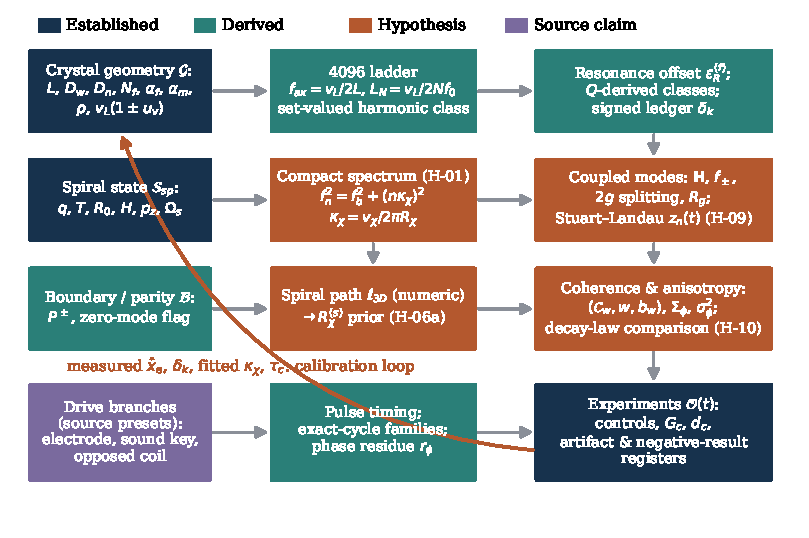
\includegraphics[width=0.98\linewidth]{fig_architecture.pdf}
\caption{RGCS v2 system architecture. Boxes are \texttt{rgcs\_core} module
groups, colored by the classification of their central content; the return
path carries measured quantities (node coordinate $\hat x_e$, correction
ledger $\delta_k$, fitted $\kchi$ and $\tau_c$) back into the forward
model.}
\label{fig:arch}
\end{figure}

\subsection{Faceted crystal geometry}\label{sec:geomfound}

For an $N_f$-sided regular section of diameter $D$ measured across
vertices \eqid{RGCS-M.1}\ \EST
\begin{equation}
A(D) = \frac{N_f}{8}\,D^2 \sin\!\frac{2\pi}{N_f},
\qquad
r_a = \frac{D}{2}\cos\!\frac{\pi}{N_f},
\end{equation}
with the across-flats convention $A(D) = N_f (D/2)^2\tan(\pi/N_f)$,
$r_a = D/2$ \eqid{RGCS-M.2--M.3}. Termination (cap) heights follow the
declared angle convention \eqid{RGCS-M.4}\ \EST:
\begin{equation*}
h = r_a\tan\alpha\ \text{(\texttt{face\_slope})},\qquad
h = \frac{r_a}{\tan\alpha}\ \text{(\texttt{axis\_to\_face})},\qquad
h = \frac{r_a}{\tan(\alpha/2)}\ \text{(\texttt{apex\_included})}.
\end{equation*}
The convention must be declared with every
dimension set; the default angle values $51.843^\circ/60^\circ$ are Source
claims \SRC\ (their numerological audit is Established arithmetic:
$\arctan\sqrt{\varphi} = \gvAngleGolden^\circ$, a nonzero
$\gvAngleDelta^\circ$ from the proposed value — the manuscript makes no
golden-ratio equality claim). Total volume is the tapered polygonal frustum
plus two pyramidal caps \eqid{RGCS-M.5}\ \EST,
\begin{equation}
V = \frac{h_s}{3}\Bigl(A_w + A_n + \sqrt{A_w A_n}\Bigr)
  + \frac{A_w h_f}{3} + \frac{A_n h_m}{3},
\qquad h_s = L - h_f - h_m > 0,
\end{equation}
and $m = \rho V$ \eqid{RGCS-M.6} with handbook density
$\rho = 2.65$\,\si{g/cm^3} for $\alpha$-quartz \citep{wardquartz}. The
density inverse — solving $\rho V(s_D D_w, s_D D_n; L) = m^\ast$ for the
diameter scale $s_D$ given a measured mass — has a unique root because $V$
is strictly increasing in $s_D$; the core solves it by guarded Newton
iteration to $|\Delta m|/m^\ast < 10^{-10}$ \eqid{RGCS-M.7}\ \DER.

\subsection{Wave propagation and the uncertain wave speed}\label{sec:wavespeed}

$\alpha$-quartz is trigonal and anisotropic
\citep{bechmann1958,wardquartz,vig1997}: from Bechmann's elastic constants,
the pure longitudinal speed along the crystallographic $Z$ axis is
$\sqrt{c_{33}/\rho} \approx 6320$\,\si{m/s}, while along $X$ it is
$\sqrt{c_{11}/\rho} \approx 5720$\,\si{m/s} \EST. The corpus value
$\vbarL = \gvVL$\,\si{m/s} is consistent with the $Z$-axis longitudinal
speed \citep{bechmann1958} but was imported uncited \SRC; RGCS therefore
treats the wave speed as a first-class uncertain parameter
\eqid{RGCS-M.10}\ \DER:
\begin{equation}
\vL = \vbarL(1 + \delta_v), \qquad \mathbb{E}[\delta_v] = 0,\qquad
\operatorname{sd}(\delta_v) = \uv = 0.05,
\end{equation}
where the default $\uv$ covers the $X$--$Z$ longitudinal spread until a
specimen's crystallographic orientation is measured, at which point $\uv$
may be reduced per specimen with cited constants. Since every ladder
frequency and length below is proportional to $\vL$, the relative
uncertainty propagates unchanged \eqid{RGCS-M.11}:
$u(f_{ax})/f_{ax} = u(L_N)/L_N = \uv$. \textbf{Interpretation rule:} any
sub-percent ``match'' to a ladder frequency is two orders of magnitude
smaller than this systematic band and is Derived-from-Hypothesis
arithmetic, never confirmation (Section~\ref{sec:ladder}).

% ======================================================================
\section{Crystal geometry and the 4096 design ladder}\label{sec:ladder}
% ======================================================================

The first-order axial half-wave estimate is \eqid{RGCS-M.8}
\begin{equation}
f_{ax} = \frac{\vL}{2L},
\qquad
L_N = \frac{\vL}{2 N f_0},
\label{eq:ladder}
\end{equation}
where the formula is Established \EST, the choice $f_0 = 4096$\,Hz is a
Source claim \SRC\ \citep{jenhanlog}, and the applicability of a pure
longitudinal 1-D model to a faceted, tapered, hand-finished crystal is
Hypothesis H-01a \HYP\ (cf.\ the extensional-mode literature for uniform
cylinders \citep{hund1930}). For $\vbarL = \gvVL$\,\si{m/s} the ladder
constant is $\gvLadderConst/N$\,mm, giving $L_5 = \gvLfive$\,mm and
$L_7 = \gvLseven$\,mm, each carrying $\pm\gvUv\%$.

\paragraph{The 110\,mm specimen, stated correctly.}
A source-referenced 110\,mm specimen yields
$f_{ax} = \gvFaxOneTen \pm \gvFaxOneTenSigma$\,Hz ($1\sigma$), which sits
$+\gvFaxOneTenErrHz$\,Hz ($+\gvFaxOneTenErrPct\%$) above $7 \times 4096 =
28672$\,Hz. The celebrated $0.03\%$ agreement is real arithmetic — and it
lives \emph{inside} a $\pm 5\%$ systematic band roughly $170\times$ wider
than the residual. It is classified Derived-from-Hypothesis-and-Source-claim
\DER: it rests on the 1-D applicability hypothesis (H-01a) and on the
source-claimed specimen length, and it is never presented as confirmation
of anything. What it does earn is a pre-registered measurement: the
specimen's actual free fundamental, against the full interval prediction.

\paragraph{Set-valued harmonic classification.}
Because the prediction is an interval, classification must be too
\eqid{RGCS-M.12}\ \DER:
\begin{equation}
\mathcal{N} = \Bigl\{\,N' \in \mathbb{N}:\ \bigl[f_{ax}(1-\uv),\,
f_{ax}(1+\uv)\bigr]\cap\bigl[(N'-\tfrac12)f_0,\ (N'+\tfrac12)f_0\bigr]
\neq \emptyset\,\Bigr\}.
\end{equation}
A 116\,mm example gives $f_{ax} = \gvFaxOneSixteen$\,Hz, $N_{\rm eff} =
\gvNeffOneSixteen$, and the \emph{ambiguous} class set $\mathcal{N} =
\gvClassSetOneSixteen$ at $\uv = 0.05$: the specimen cannot honestly be
assigned a single harmonic number from length alone
(Table~\ref{tab:worked}).

% Auto-generated by tools/make_tables.py from rgcs_core — do not edit.
\begin{table}[t]
\centering\small
\caption{Set-valued harmonic classification (RGCS-M.12) at $u_v = 0.05$,
$f_0 = 4096$ Hz. Fractional error is quoted against $N_{\rm nearest} f_0$;
by the interpretation rule (RGCS-M.11, D-04) every value here is
Derived-from-Hypothesis arithmetic, never confirmation.}
\label{tab:worked}
\begin{tabular}{@{}rrrrrccr@{}}
\toprule
$L$ (mm) & $f_{ax}$ (Hz) & $\pm1\sigma$ band (Hz) & $N_{\rm eff}$ &
nearest $N$ & class set $\mathcal{N}$ & ambiguous & error \\
\midrule
154.052734 & 20480.0 & [19456, 21504] & 5.0000 & 5 & \{5\} & no & +0.000\% \\
110.000000 & 28681.8 & [27248, 30116] & 7.0024 & 7 & \{7\} & no & +0.034\% \\
116.000000 & 27198.3 & [25838, 28558] & 6.6402 & 7 & \{6, 7\} & yes & -5.140\% \\
\bottomrule
\end{tabular}
\end{table}


% ======================================================================
\section{Spiral and conical geometry and the compact phase coordinate}\label{sec:spiral}
% ======================================================================

The spiral-cone state path is the four-component curve \eqid{RGCS-M.30}
\EST\ (differential geometry; physical relevance is Hypothesis H-06):
\begin{equation}
X(\theta) =
\begin{bmatrix}
R_0 e^{-a\theta}\cos\theta\\
R_0 e^{-a\theta}\sin\theta\\
H\bigl(1 - (r/R_0)^{p_z}\bigr)\\
\chi_0 + \Omega_s\,\theta
\end{bmatrix},
\qquad \theta \in [0,\, 2\pi T],
\qquad a = \frac{\ln q}{2\pi},
\label{eq:spiral}
\end{equation}
with growth ratio $q$ per turn, $T$ turns, outer radius $R_0$, cone height
$H$, and cone exponent $p_z$ (the $z$-law is equivalent to
$H(1 - e^{-p_z a\theta})$). The fourth coordinate reduced modulo $2\pi$ is
the compact phase $\chi$ — a modeling construct, \emph{not} a spatial extra
dimension. For $q = e$: pitch parameter $a = \gvSpiralA$
\eqid{RGCS-M.31}, planar scale-rotation eigenvalue $\lambda_s = -a + i$
\eqid{RGCS-M.32}, and curvature invariant $r\kappa = 1/\sqrt{1+a^2} =
\gvRkappa$ \eqid{RGCS-M.33}, all \EST.

\paragraph{Path length: the numeric value is authoritative.}
The exact planar arc length is
$\ell_{pl} = R_0\sqrt{1+a^2}\,(1 - e^{-2\pi a T})/a = \gvEllPl$\,mm
\eqid{RGCS-M.34}\ \EST. The \emph{project-defining} 3-D path length is the
converged numeric polyline \eqid{RGCS-M.35}\ \DER,
\begin{equation}
\ell_{3D} = \lim_{\text{refinement}} \sum_i
\bigl\lVert X_{3D}(\theta_{i+1}) - X_{3D}(\theta_i)\bigr\rVert
= \gvEllThreeD\ \text{mm},
\end{equation}
computed with sample doubling until the relative change is below $10^{-6}$.
The workbook closed form $\ell_{pl}\sqrt{1 + (H/\ell_{pl})^2}$ is
\emph{retired as a definition}: it assumes the climb is distributed
uniformly along the planar length and here evaluates to $\gvClosedForm$\,mm,
an error of $\gvClosedFormErrPct\%$ against $\ell_{3D}$ — it may appear
only as this labeled approximation with its error printed.

\paragraph{Compact-radius priors.}
Two competing definitions bridge the spiral to the compact spectrum, both
Hypothesis-classified \HYP:
\begin{equation}
R_\chi^{(s)} = \frac{\ell_{3D}}{2\pi T} = \gvRchiPrior\ \text{mm}
\quad\text{\eqid{RGCS-M.36}},
\qquad\qquad
R_{\chi,k} = \frac{\ell_k}{2\pi} = \gvPerTurnRadii\ \text{mm}
\quad\text{\eqid{RGCS-M.37}},
\end{equation}
the mean-per-turn prior (averaging assumption A-07) and the per-turn
alternative whose lengths contract by $\approx 1/q$ each turn
(Figure~\ref{fig:spiral}). The pre-registered model comparison of
Section~\ref{sec:examples} must test both against measured mode spacing;
neither is presumed. The prototype default ``$\Rchi = 100$\,mm'' is an
arbitrary placeholder unrelated to these spiral values, and the code never
presents them as consistent.

\begin{figure}[t]
\centering
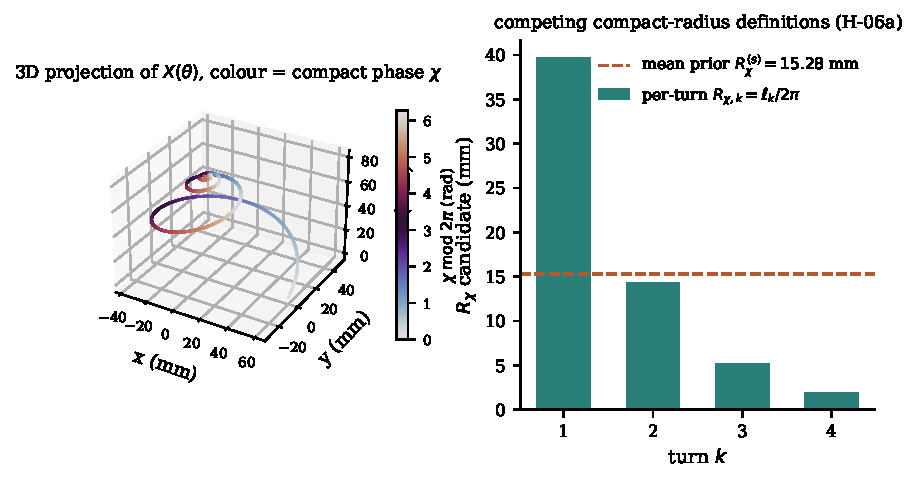
\includegraphics[width=0.98\linewidth]{fig_spiral_projection.pdf}
\caption{Left: three-dimensional projection of the four-component path
$X(\theta)$ \eqid{RGCS-M.30} for $q = e$, $T = 4$, $R_0 = 60$\,mm,
$H = 80$\,mm, $p_z = 1.5$, colored by the compact phase coordinate $\chi
\bmod 2\pi$. Right: the two competing compact-radius definitions; the
per-turn radii contract by $\approx 1/q$ per turn, so the mean prior hides
real structure that the model comparison of H-06a must adjudicate.}
\label{fig:spiral}
\end{figure}

% ======================================================================
\section{Compact-coordinate mode spectrum}\label{sec:compact}
% ======================================================================

\subsection{The spectrum and its substitution map}

RGCS v2 posits a closed wave path of effective radius $\Rchi$ supporting
propagation at speed $\vchi$, with mode spectrum \eqid{RGCS-M.13}\ \HYP\
(Hypothesis H-01, built on Established Kaluza--Klein mode algebra):
\begin{equation}
f_n^{2} = \fb^{2} + \Bigl(\frac{n\,\vchi}{2\pi \Rchi}\Bigr)^{2}.
\label{eq:compact}
\end{equation}
Equation~\eqref{eq:compact} is a direct mathematical adaptation of the
tree-level dark-photon mass formula of \citet[Eqs.~(9)--(10)]{leetsai2026},
$m_{\gamma_D}^{(n)} = \sqrt{m_B^2 + n^2/R^2}$, under the explicit
substitution map
\begin{equation*}
m \longrightarrow f,\qquad
m_B \longrightarrow \fb,\qquad
\frac{1}{R} \longrightarrow \frac{\vchi}{2\pi \Rchi},
\end{equation*}
which is dimensionally exact for wave propagation around a circumference
$2\pi\Rchi$. The massless-base limit $\fb = 0$ reproduces their fermion
tower $m_E^{(n)} = n/R$ \citep[Eq.~(9)]{leetsai2026}. The physical claim —
that any measured RGCS mode family obeys Eq.~\eqref{eq:compact} better than
simpler modal models on held-out modes — is Hypothesis H-01 with a
pre-registered failure condition (Section~\ref{sec:roadmap}). RGCS's
$\chi$ is a closed wave path; nothing here asserts an extra spatial
dimension of a crystal.

\subsection{Identifiability: report \texorpdfstring{$\kchi$}{kappa}, not \texorpdfstring{$(\vchi, \Rchi)$}{(v,R)}}

Only the combination \eqid{RGCS-M.14}\ \DER
\begin{equation}
\kchi \equiv \frac{\vchi}{2\pi \Rchi}\qquad[\text{Hz}]
\end{equation}
enters Eq.~\eqref{eq:compact}: $\vchi$ and $\Rchi$ are \emph{not separately
identifiable} from mode spacing alone. Fits report $\kchi$ with
uncertainty; $\Rchi$ is quoted only when $\vchi$ is independently fixed
(e.g., $\vchi := \vL$ with its $\uv$), and then $u(\Rchi)/\Rchi \ge \uv$
necessarily. The spiral prior of Section~\ref{sec:spiral} breaks the
degeneracy only under Hypothesis H-06a. With $\vchi = \vbarL$ and the
placeholder $\Rchi = 100$\,mm, $\kchi = \gvKappaChi$\,Hz and the $n = 1$
mode is the golden value $\gvCompactN$\,Hz~$\pm 5\%$; with the spiral prior
$R_\chi^{(s)} = \gvRchiPrior$\,mm instead, $\kchi \approx
\gvKappaPrior$\,Hz — the two differ by a factor of $\sim$6.5, which is
precisely why the placeholder is labeled a placeholder. First-order
uncertainty propagation \eqid{RGCS-M.15} makes every spectrum output an
interval (Table~\ref{tab:compact}, Figure~\ref{fig:ladderfig}).

% Auto-generated by tools/make_tables.py from rgcs_core — do not edit.
\begin{table}[t]
\centering\small
\caption{Compact-coordinate spectrum for $f_b = 0$,
$\kappa_\chi = 10042.68$ Hz $\pm5\%$
($v_\chi = \bar v_L$, $R_\chi = 100$ mm placeholder, D-21). The $n = 0$
member is excluded unconditionally at $f_b = 0$ (RGCS-M.17). Intervals are
the mandatory $\pm u_v$ propagation of RGCS-M.15.}
\label{tab:compact}
\begin{tabular}{@{}rlrr@{}}
\toprule
$n$ & parity & $f_n$ (Hz) & $\pm1\sigma$ band (Hz) \\
\midrule
1 & odd & 10042.68 & [9541, 10545] \\
2 & even & 20085.35 & [19081, 21090] \\
3 & odd & 30128.03 & [28622, 31634] \\
4 & even & 40170.71 & [38162, 42179] \\
5 & odd & 50213.38 & [47703, 52724] \\
6 & even & 60256.06 & [57243, 63269] \\
\bottomrule
\end{tabular}
\end{table}


\begin{figure}[t]
\centering
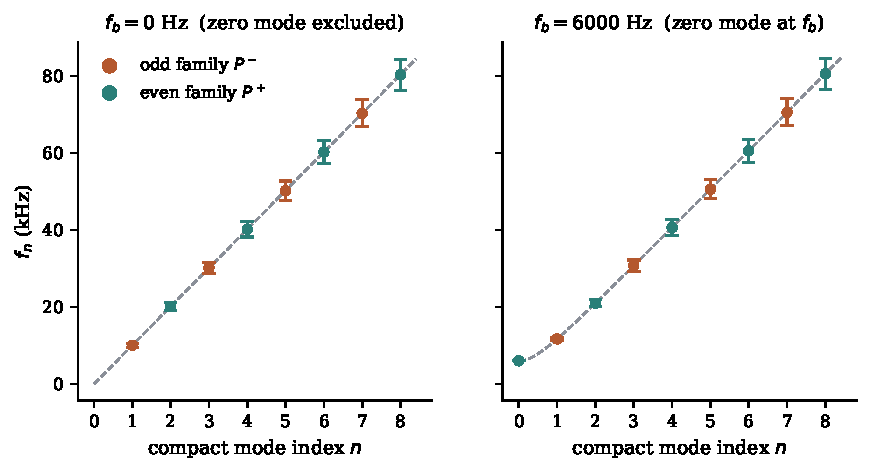
\includegraphics[width=0.98\linewidth]{fig_compact_ladder.pdf}
\caption{Compact-mode ladder \eqid{RGCS-M.13} with mandatory $\pm\uv$
uncertainty bands, for a massless base ($\fb = 0$, left; linear in $n$, the
\citet{leetsai2026} fermion-tower limit, zero mode excluded unconditionally)
and a finite base frequency ($\fb = 6$\,kHz, right; quadrature form with
the $n = 0$ member at $\fb$). Colors distinguish the odd and even parity
families of Section~\ref{sec:parity}.}
\label{fig:ladderfig}
\end{figure}

\subsection{Boundary parity and the zero-mode rule}\label{sec:parity}

On a compact coordinate with two distinguished boundary points, mode
functions divide into parity families \eqid{RGCS-M.16}\ \EST\ (as index-set
definitions; their physical relevance to RGCS resonators is Hypothesis
H-03):
\begin{equation}
u_n^-(\chi) \propto \sin\frac{n\chi}{2},\ n \in \mathbb{I}^- = \{1,3,5,\dots\},
\qquad
u_n^+(\chi) \propto \cos\frac{n\chi}{2},\ n \in \mathbb{I}^+ = \{0,2,4,\dots\},
\end{equation}
adapted from the boundary-condition classification of
\citet[Table~I, Eqs.~(1)--(2)]{leetsai2026}, where orbifold conditions
select odd fermion and even dark-photon modes. In RGCS, odd means an
antisymmetric displacement/current/pressure pattern about the reference
plane and even means symmetric; assignment is made by two-sensor phase or
finite-element mode shape, \emph{never} by which family contains a desired
frequency (Figure~\ref{fig:parity}).

The zero mode requires care \eqid{RGCS-M.17}\ \DER. The odd family never
contains $n = 0$ ($\sin \equiv 0$ is not a mode). The even family contains
$n = 0$ mathematically, with $f_{n=0} = \fb$; in the strict Lee--Tsai
template a zero-flux condition removes the mediator zero mode
\citep[Eq.~(2)]{leetsai2026}. RGCS therefore exposes an explicit boolean
\texttt{include\_zero\_mode} on the even family: \texttt{True} (default when
$\fb > 0$) lists the physical base mode; \texttt{False} reproduces the
strict template for exact-analogy tests. When $\fb = 0$ the $n = 0$ member
is a DC pattern and is excluded unconditionally. \textbf{Every spectrum in
this manuscript that cites \citet{leetsai2026} states its flag} (all
figures and tables here use \texttt{include\_zero\_mode = True} except
where marked), and a measured low-lying symmetric mode where the strict
template forbids one is pre-registered evidence that the analogy is partial
(H-04).

\begin{figure}[t]
\centering
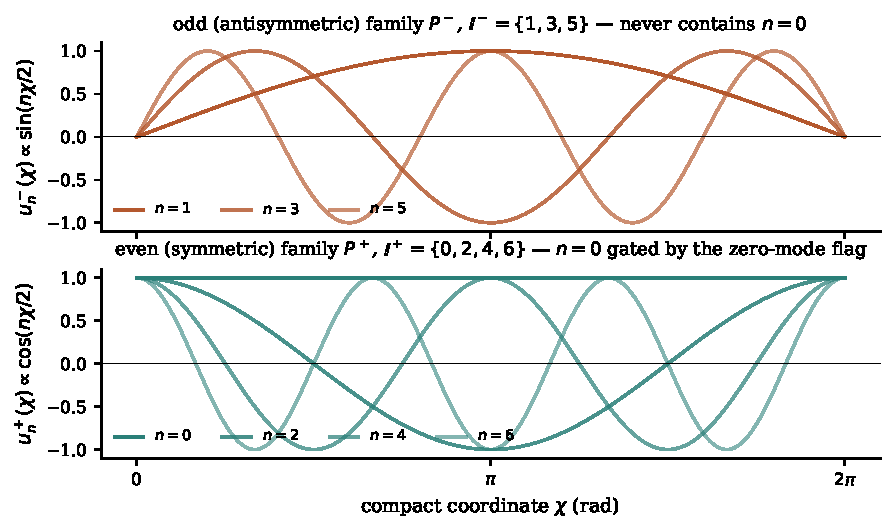
\includegraphics[width=0.92\linewidth]{fig_parity_families.pdf}
\caption{Parity families \eqid{RGCS-M.16} on the compact coordinate,
adapted from \citet[Table~I]{leetsai2026}. Zero-mode flag:
\texttt{include\_zero\_mode = True} (the $n=0$ even member is drawn;
under the strict Lee--Tsai template it would be removed by the zero-flux
condition).}
\label{fig:parity}
\end{figure}

% ======================================================================
\section{Resonance-offset functional}\label{sec:offset}
% ======================================================================

\subsection{Definition and sign convention}

For a measured bridge (mediator-like) mode $f_m$ and target (matter-like)
mode $f_x$ with pair multiple $p$ (default 2), RGCS defines
\eqid{RGCS-M.18}\ \DER
\begin{equation}
\epsR = \frac{f_m^2 - (p f_x)^2}{(p f_x)^2},
\label{eq:epsf}
\end{equation}
with sign convention identical to the resonance level of
\citet[Eq.~(13)]{leetsai2026}: $\epsR > 0$ places the bridge above the
threshold, $\epsR < 0$ below. Their invisible/visible dark-photon
interpretation of the sign has \emph{no} RGCS analogue. The conjecture
that transfer or splitting enhancement localizes near $\epsR = 0$ is
Hypothesis H-02 \HYP. For small detunings, $\epsR = (1 + d_{\rm lin})^2 -
1 \approx 2 d_{\rm lin}$ with $d_{\rm lin} = f_m/(p f_x) - 1$
\eqid{RGCS-M.19}\ \EST.

\subsection{\texorpdfstring{$Q$}{Q}-derived proximity classes}

Earlier drafts borrowed the window $10^{-8} \le \epsilon_R \le 10^{-4}$
from the dark-sector context \citep{leetsai2026}; that window is
astrophysics, not metrology, and is retired. RGCS classes now derive from
measured linewidths \eqid{RGCS-M.20}\ \DER: a mode pair with effective
quality factor $Q_{\rm eff} = 2/(1/Q_m + 1/Q_x)$ has fractional
half-linewidth scale
\begin{equation}
\epsilon_Q \equiv \frac{1}{Q_{\rm eff}},
\end{equation}
and the classes are \textsc{within linewidth} ($|\epsR| \le \epsilon_Q$),
\textsc{near} ($\le 5\epsilon_Q$), \textsc{moderate} ($\le 50\epsilon_Q$),
and \textsc{far} otherwise. For $Q_m = 1000$, $Q_x = 800$:
$\epsilon_Q = \gvEpsQ$ — resolvable by ordinary instrumentation, unlike the
retired bins. A resonance-class string reported without $u(\epsR)$ is
non-compliant (Table~\ref{tab:classes}, Figure~\ref{fig:epsmap}). The
far-detuned reference $\epsilon = 1.25$ — the value at which the
Lee--Tsai mediator sits at three times the pair threshold
\citep{leetsai2026} — is retained \emph{only} as the convention defining a
deliberately non-resonant control configuration; it is a control
convention, not physics.

% Auto-generated by tools/make_tables.py from rgcs_core — do not edit.
\begin{table}[t]
\centering\small
\caption{$Q$-derived resonance classes (RGCS-M.20) for a target mode
$f_x = 20480$ Hz, $p = 2$, $Q_m = 1000$, $Q_x = 800$
($\epsilon_Q = 1/Q_{\rm eff} = \num{1.125e-03}$). A class string without
$u(\epsilon_R)$ is non-compliant (policy \S3.4). Sweep spans include the
six-linewidth floor of RGCS-M.21 (engineering heuristic).}
\label{tab:classes}
\begin{tabular}{@{}rrrlr@{}}
\toprule
$f_m$ (Hz) & $\epsilon_R^{(f)}$ & $u(\epsilon_R)$ & class & sweep span (Hz) \\
\midrule
40960 & +0.00000 & \num{2e-04} & within linewidth & 246 \\
40970 & +0.00049 & \num{2e-04} & within linewidth & 246 \\
41100 & +0.00685 & \num{2e-04} & moderate & 560 \\
41800 & +0.04144 & \num{3e-04} & moderate & 3360 \\
45000 & +0.20699 & \num{5e-04} & far & 16160 \\
61440 & +1.25000 & \num{1e-03} & far & 81920 \\
\bottomrule
\end{tabular}
\end{table}


\begin{figure}[t]
\centering
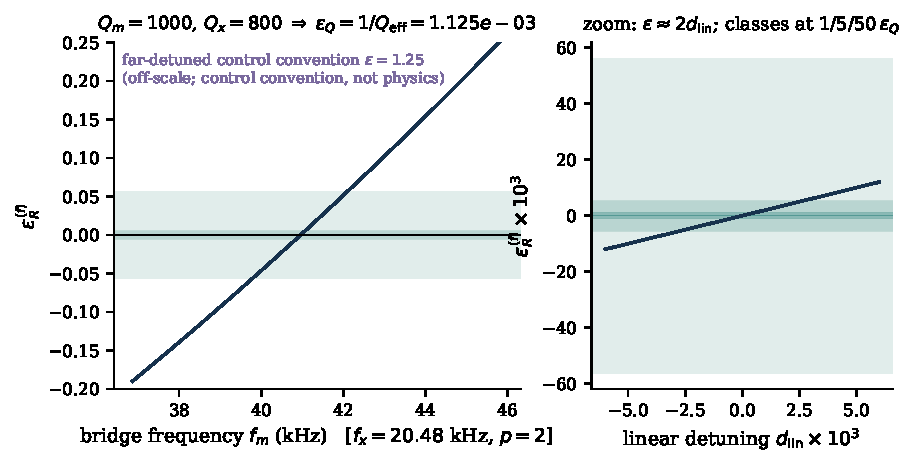
\includegraphics[width=0.98\linewidth]{fig_epsilon_map.pdf}
\caption{Resonance-offset functional \eqid{RGCS-M.18} and $Q$-derived
classes \eqid{RGCS-M.20} for $f_x = 20480$\,Hz, $p = 2$, $Q_m = 1000$,
$Q_x = 800$. Shaded bands mark the \textsc{within-linewidth}, \textsc{near},
and \textsc{moderate} classes at $1/5/50 \times \epsilon_Q$; sign convention
follows \citet[Eq.~(13)]{leetsai2026}.}
\label{fig:epsmap}
\end{figure}

\subsection{Corrections shift the offset — with sign}

The Lee--Tsai one-loop corrections \citep[Eqs.~(11)--(12)]{leetsai2026}
carry definite signs and can move $\epsilon_R$ through zero; RGCS's
calibration analogue is the signed correction ledger \eqid{RGCS-M.22,
M.45}\ \DER
\begin{equation}
f_{i,\rm corr} = f_{i,0}\Bigl(1 + \sum_k \delta_k^{(i)}\Bigr),
\qquad
u(\epsR)\big|_{\epsilon\approx0} \approx
2\sqrt{\Bigl(\frac{u(f_m)}{f_m}\Bigr)^{2} +
\Bigl(\frac{u(f_x)}{f_x}\Bigr)^{2}},
\end{equation}
with $\delta_k \in \{\delta_{\rm geometry}, \delta_{\rm anisotropy},
\delta_{\rm loading}, \delta_T, \delta_{\rm fixture}, \delta_{\rm drive}\}$
each signed and carrying its own uncertainty. A worked ledger example
(loading $-0.4\%$, temperature $+0.08\%$ on $f_m$; fixture $+0.1\%$ on
$f_x$) moves an exactly-zero offset to $\epsR = \gvCorrEps \pm
\gvCorrEpsU$: through zero and out the other side. Repeated $\delta_k$
measurements must be stable across calibrations before any $\epsR$ is
interpreted — this gates Hypothesis H-02.

% ======================================================================
\section{Coupled eigenmodes and avoided crossings}\label{sec:coupled}
% ======================================================================

Two modes with uncoupled frequencies $f_A, f_B$ and coupling $g$ obey the
standard symmetric two-mode model \eqid{RGCS-M.23--M.25}\ \EST\
\citep{novotny2010}:
\begin{equation}
\mathbf{H} = \begin{bmatrix} f_A & g\\ g & f_B \end{bmatrix},
\qquad
f_\pm = \frac{f_A + f_B}{2} \pm
\sqrt{\Bigl(\frac{f_A - f_B}{2}\Bigr)^{2} + g^{2}},
\qquad
\vartheta_{\rm mix} = \tfrac12\operatorname{atan2}(2g,\ f_A - f_B).
\end{equation}
At zero detuning the splitting is $2g$ (golden value: $f_A = f_B =
1000$\,Hz, $g = 10$\,Hz $\Rightarrow$ $\gvHybridLo/\gvHybridHi$\,Hz). With
FWHM linewidths $\Gamma_n = f_n/Q_n$ \eqid{RGCS-M.26} the strong-coupling
criterion is \eqid{RGCS-M.27}\ \EST\ \citep{novotny2010,aspelmeyer2014}
\begin{equation}
R_g = \frac{2g}{\Gamma_A + \Gamma_B} \gtrsim 1
\quad\Longleftrightarrow\quad
\text{splitting resolved against the combined linewidth}.
\end{equation}
Figure~\ref{fig:avoided} shows the worked case $f_B = 20480$\,Hz,
$g = 25$\,Hz, $Q = 1000$: splitting $2g = \gvACSplit$\,Hz against
$\Gamma = \gvACGamma$\,Hz per mode, $R_g = \gvACRg$ — just resolved. A
resolved anticrossing is a far stronger signature than a single coincident
peak. The $N$-mode generalization \eqid{RGCS-M.28} is a real symmetric
eigenproblem (orthogonal eigenvectors, \texttt{numpy.linalg.eigh}), valid
in the near-degenerate weak-coupling regime; it is \emph{not} a substitute
for full elastodynamics.

\paragraph{Geometry scaling of the coupling.} The Lee--Tsai dimensional
reduction $g_1 = g_1^{(5)}/\sqrt{L}$ \citep[Eq.~(6)]{leetsai2026} motivates
the testable scaling \eqid{RGCS-M.29}\ \HYP\ (H-05)
\begin{equation}
g \propto (2\pi \Rchi)^{-1/2}
\quad\text{at fixed transducer and mode pair};
\end{equation}
a fitted $g$ that fails to scale as $\sqrt{R_2/R_1}$ after a controlled
compact-path change kills this analogy row.

\begin{figure}[t]
\centering
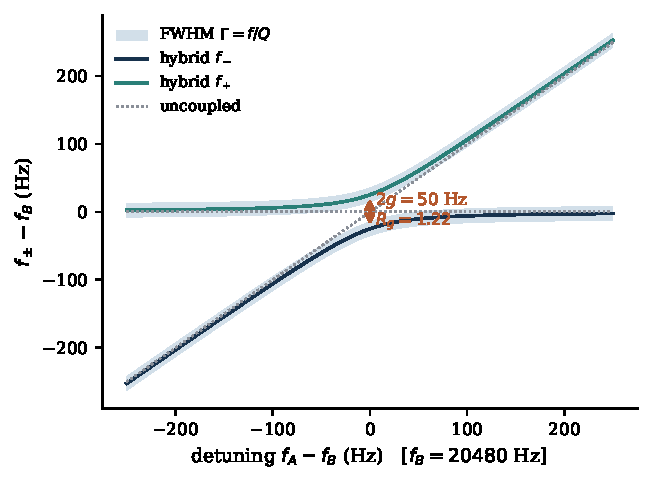
\includegraphics[width=0.62\linewidth]{fig_avoided_crossing.pdf}
\caption{Avoided crossing \eqid{RGCS-M.24} for a fixed mode at
$20480$\,Hz coupled with $g = 25$\,Hz to a swept mode ($Q_A = Q_B = 1000$).
Shaded bands are the FWHM linewidths; the minimum splitting $2g$ against
the combined linewidth gives $R_g = \gvACRg$.}
\label{fig:avoided}
\end{figure}

% ======================================================================
\section{Node, loading, damping, and correction models}\label{sec:node}
% ======================================================================

\subsection{Node coordinate (female-apex frame)}

The corpus distinguishes a functional (``vorticial'') node from the metric
center \SRC. RGCS stores three quantities in the declared frame ($x$ from
the female apex) \eqid{RGCS-M.38--M.40}:
\begin{equation}
x_m = \frac{L}{2},
\qquad
x_g = h_f + \frac{h_s}{2} = \frac{L + h_f - h_m}{2},
\qquad
\hat x_e = \text{measured node coordinate},
\end{equation}
where $x_g$ \DER\ applies the free--free uniform-bar midpoint principle to
the prismatic shaft and is a \emph{prior only}, and a measured $\hat x_e$
always takes precedence. For the default $N = 5$ geometry ($L =
\gvLfive$\,mm, $h_f = \gvHf$\,mm, $h_m = \gvHm$\,mm): $x_g = \gvXg$\,mm
versus $x_m = \gvXm$\,mm. The historical 75.725\,mm estimate is exactly
$L - x_g = \gvXgMale$\,mm — the same point expressed from the male apex, a
frame conversion, not a competing estimator; a third legacy estimator with
no derivation was deleted from the code. The node-alignment factor
$N_x = \exp[-((x_d - x_\ast)/\sigma_x)^2]$ \eqid{RGCS-M.41} is an
engineering heuristic feeding only the merit score, never evidence.

\subsection{Loading}

The loading factor is the measured ratio \eqid{RGCS-M.42}\ \EST\
$k_H = f_{\rm loaded}/f_{\rm free}$, a long-standing quartz measurement
problem \citep{sogn1952,vig1997}. Under Hypothesis H-08 — that loading
acts as pure added modal mass with modal fraction $\eta$ — first-order
SDOF algebra gives \eqid{RGCS-M.43}
\begin{equation}
\Delta M_H = M_{\rm eff}\Bigl(\frac{1}{k_H^{2}} - 1\Bigr),
\qquad M_{\rm eff} = \eta\, m .
\end{equation}
Golden example: $k_H = \gvKH$ (the $152/\gvLfive$ ratio), $m = 154$\,g,
$\eta = 0.5$ $\Rightarrow$ $\Delta M_H = \gvDMH$\,g — conditioned on the
\emph{unmeasured} $\eta$, whose scale degeneracy with $\Delta M_H$ requires
either fixing $\eta$ or a two-loading protocol. The length-shortfall proxy
$\tilde k_H = L_{\rm actual}/L_{\rm target}$ \eqid{RGCS-M.44}\ \HYP\
(H-08b) is a \emph{distinct} quantity: it equals $k_H$ only if $f \propto
1/L$ exactly and loading is intended to close the gap; code and text keep
the tilde.

\subsection{Damping and the correction ledger}

Modal damping follows from measured quality factors \eqid{RGCS-M.49}\ \EST:
$\gamma_n = \omega_n/(2 Q_n)$ (amplitude decay; energy decays at
$2\gamma_n$). The full measurement model \eqid{RGCS-M.45, M.59} is
\begin{equation}
f_{\rm meas} = f_{0,\rm pred}\Bigl(1 + \textstyle\sum_k \delta_k\Bigr)
+ \varepsilon_{ns},
\end{equation}
first-order additive (a nonlinear or Bayesian treatment supersedes it when
$|\sum\delta| > 0.02$), with independent Gaussian noise
$\varepsilon_{ns}$; fits minimize the standard negative log-likelihood with
bootstrap checks at small $n$ \citep{efron1979}.

% Auto-generated by tools/make_tables.py from rgcs_core — do not edit.
\begin{table}[t]
\centering\small
\caption{Spiral-path and node-coordinate worked example. Spiral defaults
$q = e$, $T = 4$, $R_0 = 60$ mm, $H = 80$ mm, $p_z = 1.5$; crystal
$L = 154.052734$ mm, $D_w/D_n = 32/25$ mm, $N_f = 6$,
$\alpha_f/\alpha_m = 51.843^\circ/60^\circ$ (angle values are Source claims);
node rows use the corpus default cap heights $h_f = 17.415434$ mm,
$h_m = 14.812763$ mm. Node coordinates are in the female-apex frame
($x$ measured from the wide apex).}
\label{tab:spiralnode}
\begin{tabular}{@{}p{0.47\linewidth} p{0.30\linewidth} l@{}}
\toprule
quantity & value (live) & status \\
\midrule
pitch parameter $a = \ln q/2\pi$ & 0.159154943 & Established \\
curvature invariant $r\kappa$ & 0.987570492 & Established \\
exact planar arc length $\ell_{pl}$ & 374.744 mm & Established \\
\textbf{numeric 3D path length $\ell_{3D}$ (authoritative)} & \textbf{384.022 mm} (converged to $10^{-6}$) & Derived \\
retired closed form $\ell_{pl}\sqrt{1+(H/\ell_{pl})^2}$ & 383.188 mm (-0.22\% vs $\ell_{3D}$) & labelled approximation \\
mean compact-radius prior $R_\chi^{(s)} = \ell_{3D}/2\pi T$ & 15.280 mm & Hypothesis (A-07) \\
per-turn radii $R_{\chi,k} = \ell_k/2\pi$ & 39.68, 14.30, 5.22, 1.92 mm & Hypothesis (alt.) \\
metric centre $x_m = L/2$ & 77.0264 mm & Established \\
node prior $x_g = (L + h_f - h_m)/2$ (female frame) & 78.3277 mm & Derived (prior only) \\
same point, male frame $L - x_g$ & 75.7250 mm & frame conversion \\
\bottomrule
\end{tabular}
\end{table}


% ======================================================================
\section{Dynamic coherence and phase evolution}\label{sec:coherence}
% ======================================================================

Version 1 was static. Version 2 adds the time axis: how a drive populates
modes, how phase order can (or cannot) emerge, and how amplitude and phase
order decay — with one normative rule imported from the measurement
architecture of \citet{koster2026}:

\begin{center}
\colorbox{soft}{\parbox{0.9\linewidth}{\small\textbf{Amplitude and
coherence are separate observables.} High amplitude is not evidence of
phase order, and phase order can outlive detectable amplitude. Every
dynamic RGCS measurement reports both, and every coherence value ships as
the triplet $(\Cw, w, b_w)$: the value, its analysis window, and the
measured noise baseline for that window. \EST\ (metric property).}}
\end{center}

\subsection{Amplitude--phase dynamics}\label{sec:dynamics}

The modal state evolves under the canonical complex system
\eqid{RGCS-M.46}\ \HYP\ (H-09; the mathematical structure — the
slowly-varying-envelope / Stuart--Landau normal form near a Hopf
bifurcation — is Established \citep{guckenheimer1983,pikovsky2001}):
\begin{equation}
\dot z_n = (G_n - \gamma_n + i\omega_n)\, z_n
- \sum_m \beta_{nm} |z_m|^2 z_n
+ \sum_m K_{nm}\, z_m ,
\label{eq:sl}
\end{equation}
with drive gain $G_n$, damping $\gamma_n = \omega_n/2Q_n$, cubic
saturation $\beta_{nm}$, and linear inter-mode coupling $K_{nm}$ — the
time-domain counterpart of the frequency-domain $g_{nm}$ is the
anti-Hermitian coupling $K_{nm} = i\,2\pi g_{nm}$ ($g$ in Hz): at
degeneracy the pair eigenvalues are $i(\omega_0 \pm 2\pi g)$, producing
spectral peaks at $f_0 \pm g$ — the $2g$ splitting of
Sec.~\ref{sec:coupled} — whereas a real-symmetric $K$ of equal magnitude
splits growth rates, not frequencies. The pre-registered consistency
requirement is $|K_{nm}| = 2\pi g_{nm}$: disagreement between
time-domain and frequency-domain coupling estimates
beyond $2\sigma$ is an internal-inconsistency flag. The polar
decomposition \eqid{RGCS-M.47--M.48} gives the amplitude and phase
equations
\begin{equation}
\dot A_n = (G_n - \gamma_n) A_n - \sum_m \beta_{nm} A_m^2 A_n
+ \sum_m K_{nm} A_m \cos(\phi_m - \phi_n),
\qquad
\dot\phi_n = \omega_n + \sum_m K_{nm}\frac{A_m}{A_n}\sin(\phi_m - \phi_n),
\end{equation}
integrated in the complex form (the polar form is singular as $A \to 0$).
Registered alternatives (full linear equations, Van der Pol gain,
sin-bounded saturation, parametric $f/2$ terms for the parametric drive
branch only, Kuramoto phase-only) are documented with the reasons each is
not the default; the linear null $\beta = K = 0$ is the model-comparison
baseline for H-09.

\subsection{The four-stage template and spontaneity}

\citet{koster2026} observe four temporal stages in a parametrically pumped
magnon gas: incoherent pair injection with no global phase (high amplitude,
baseline coherence); nonlinear redistribution; emergence of per-run-stable
phase \emph{with ensemble-uniform phase across 1{,}000 runs} — order that
is spontaneous, not drive-imprinted; and free post-drive evolution in which
coherence persists below the amplitude noise floor. RGCS adopts the
\emph{stage structure} as an analysis template (their physics stays theirs
\SRC): stage labels are assigned only from the measured (amplitude,
coherence, ensemble-phase) triple, never assumed. The spontaneity test is
the Rayleigh statistic \eqid{RGCS-M.61}\ \EST\ \citep{mardia2000} on
one phase per run,
\begin{equation}
\bar R = \Bigl|\frac{1}{n_s}\sum_{\rm shots} e^{i\phi_{\rm shot}}\Bigr|,
\qquad Z_R = n_s \bar R^{2}:
\end{equation}
uniform ensemble phase with high per-shot coherence indicates spontaneous
ordering; ensemble phase locked to the drive indicates a driven response,
and ``spontaneous'' vocabulary is forbidden for that result (H-13).

\subsection{The coherence metric}

From the phase-referenced analytic signal $z(t) = z_I + i z_Q$
\eqid{RGCS-M.55}\ \EST\ \citep{gabor1946,koster2026}, the windowed
autocorrelation coherence is \eqid{RGCS-M.56}\ \EST\ (exact adaptation of
the \citealp{koster2026} Methods definition):
\begin{equation}
\Cw(t) = \mathcal{N}_w \int d\tau\,
\Bigl|\bigl[(\bar z\,\Pi_{t,w}) \star (z\,\Pi_{t,w})\bigr](\tau)\Bigr|,
\label{eq:coherence}
\end{equation}
with boxcar window $\Pi_{t,w}$ and $\mathcal{N}_w$ normalizing a perfect
tone to 1. Properties: $\Cw \in [0,1]$; pure tone $\to 1$; white noise
$\to$ a small positive window-dependent baseline
$b_w \approx (2\sqrt{\pi}/3)/\sqrt{N_w}$ ($= \gvBaselineNw$ for the
project-default $N_w = \gvNw$ samples), which is \emph{measured per
pipeline} and reported with every value — the $\approx 0.2$ baseline of
\citet{koster2026} is their pipeline's, never reused. Their 100\,ns window
at GHz carriers maps to the same tens-of-carrier-cycles compromise chosen
per apparatus; a window-length sensitivity scan over at least three window
lengths is mandatory. Figure~\ref{fig:cohamp} demonstrates the central
metric property on the golden decaying-tone dataset: the coherence trace
holds $\Cw \approx \gvCaseCCohLate$ — well above $b_w$ — while the
amplitude has fallen to $\gvCaseCAmpLatePct\%$ of its peak. This is why
every archival ``no effect'' branch is re-adjudicated with coherence
analysis before its null is accepted (H-14), and why any null adjudicated
on amplitude alone is labeled \emph{amplitude-null, coherence-untested}.

\begin{figure}[t]
\centering
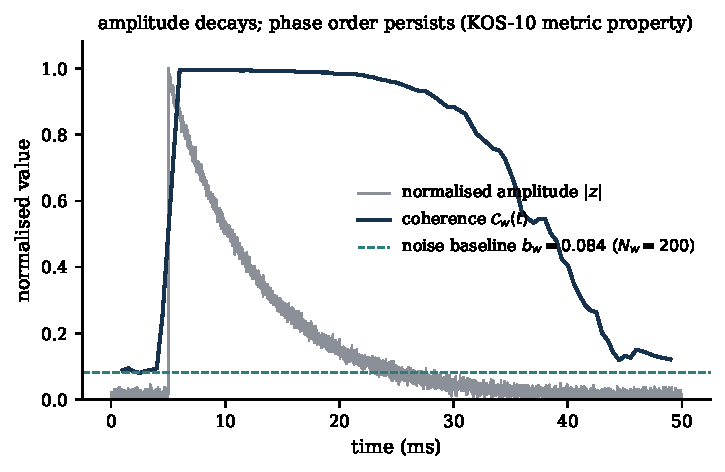
\includegraphics[width=0.72\linewidth]{fig_coherence_vs_amplitude.pdf}
\caption{Coherence versus amplitude on golden dataset (c) (decaying tone in
noise; Derived synthetic record). The autocorrelation coherence
\eqid{RGCS-M.56} persists far above the measured baseline $b_w$ after the
amplitude has decayed into the noise floor — the
\citet{koster2026} metric property that motivates coherence
re-adjudication of all amplitude-null archival results (H-14).}
\label{fig:cohamp}
\end{figure}

\begin{figure}[t]
\centering
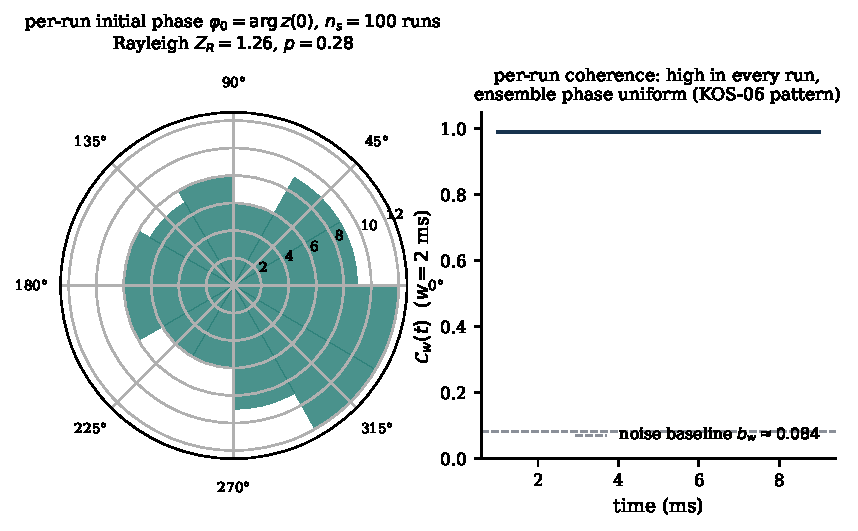
\includegraphics[width=0.95\linewidth]{fig_phase_randomization.pdf}
\caption{Phase randomization to coherence, golden dataset (d):
$\gvCaseDRuns$ synthetic runs with seeded random initial phases. Left:
ensemble initial-phase histogram with Rayleigh test
($Z_R = \gvCaseDRayZ$, $p = \gvCaseDRayP$ — consistent with uniformity).
The per-run initial phase is the unified estimator
$\varphi_0 = \arg z(0) \bmod 2\pi$
(\texttt{rgcs\_core.coherence.initial\_phase\_estimate}), used
identically here, in Table~\ref{tab:goldencoh}, and in the body text.
Right: per-run coherence traces (mean $\gvCaseDCoh$). High per-run
coherence with uniform ensemble phase is the pre-registered signature
pattern of spontaneous (non-imprinted) order; the companion pump-leakage
dataset (f) shows the trap: ensemble uniformity rejected at
$p = \num{\gvCaseFRayP}$, blocking any spontaneity claim.}
\label{fig:phaserand}
\end{figure}

% ======================================================================
\section{Spatial anisotropy and coherence damping}\label{sec:anisotropy}
% ======================================================================

\subsection{Per-axis phase rates and the anisotropy scalar}

Three orthogonal sensor channels $j = 1, 2, 3$ aligned to declared
specimen axes yield analytic signals with instantaneous phases
$\phi_j(t)$ and windowed phase rates $\Omega_j(t) = d\phi_j/dt$
\eqid{RGCS-M.51}\ \DER. The \emph{spatial phase anisotropy} scalar is
\eqid{RGCS-M.52}\ \EST\ (definition):
\begin{equation}
\sigma_\phi^{2}(t) = \frac{1}{3}\bigl[\Omega_{12}^{2} + \Omega_{23}^{2} +
\Omega_{31}^{2}\bigr],
\qquad \Omega_{jk} = \Omega_j - \Omega_k,
\label{eq:shear}
\end{equation}
an exact adaptation of the cosmological shear scalar of
\citet[Eq.~(2)]{gan2025}, $\sigma^2 = \tfrac13(H_{12}^2 + H_{23}^2 +
H_{31}^2)$, under the substitution map $H_i \rightarrow \Omega_j$
(directional Hubble rates $\to$ per-axis instantaneous phase rates). In
RGCS, Eq.~\eqref{eq:shear} is a measured statistic of bench data and
nothing more; it is zero iff all three channels evolve identically,
permutation-invariant, and insensitive to a common rate. Following the
kinematic decomposition lesson of \citet{gan2025}, the isotropic mean rate
$\Theta_\phi = (\Omega_1 + \Omega_2 + \Omega_3)/3$ is always reported
alongside, with $\sigma_\phi^2/\Theta_\phi^2$ the dimensionless anisotropy.
The companion circular-variance tensor
$\Sigma_{\phi,jk}(t) = 1 - |\langle e^{i(\phi_j - \phi_k)}\rangle_w|$
\eqid{RGCS-M.53}\ \DER\ \citep{mardia2000} captures relative-phase
\emph{locking} (0 = locked, 1 = uniformly random) with scalar reduction
$\bar\Sigma_\phi$.

\subsection{Relaxation is a model to test, not to presume}

\citet[Eq.~(6)]{gan2025} find that after the quantum bounce their shear
decays exponentially, $\sigma^2(t) \simeq \sigma_0^2\, e^{-\sigma_1 t}$
with $\sigma_1 \simeq 2.498\, m_{\rm Pl}$ — a Planck-scale, model-specific
coefficient that is dimensionally meaningless for crystals and is never
imported. RGCS adapts the \emph{form} as one member of a pre-registered
model set \eqid{RGCS-M.54}\ \HYP\ (H-10):
\begin{equation}
M_{\exp}:\ \bar\Sigma_\phi(t) = \bar\Sigma_{\phi,0}\, e^{-t/\tau_c},
\qquad
M_0:\ \text{const},
\qquad
M_{\rm pl}:\ \bar\Sigma_{\phi,0}(1 + t/t_0)^{-\alpha},
\qquad
M_{\rm se}:\ \bar\Sigma_{\phi,0}\, e^{-(t/\tau_c)^{\beta_s}},
\end{equation}
adjudicated by AIC/BIC \citep{akaike1974,schwarz1978} on post-drive
ringdown windows, mirroring the three-model comparison layout of
\citet{gan2025} (their GR / LQC / mLQC-I contrast becomes our
no-decay-null / power-law / exponential contrast). The no-decay null
mirrors their classical conserved-shear baseline. $\tau_c$ is a fitted
bench parameter, specimen- and branch-specific; whether $\tau_c$ is
\emph{independent of drive branch} at matched energy — the bench analogue
of their matter-independence result, adopted purely as a test-design
pattern — is the separate Hypothesis H-11.

Figure~\ref{fig:aniso} demonstrates the full pipeline on a seeded
synthetic three-channel record with known exponential ground truth
($\tau_c^{\rm truth} = \gvAnisoTauTruthMs$\,ms for the squared scalar):
the exponential model wins with $\Delta\mathrm{AIC} = \gvAnisoDAICNull$
over the no-change null and $\Delta\mathrm{AIC} = \gvAnisoDAICDamped$ over
the damped-oscillatory alternative, and the fitted
$\tau_c = \gvAnisoTauMs$\,ms recovers the truth within $3\%$. On real
data, support for H-10 additionally requires $\Delta\mathrm{AIC} \ge 4$
against the null \emph{and} $\tau_c$ stability across same-specimen
repeats, with a mandatory window-sensitivity scan.

\begin{figure}[t]
\centering
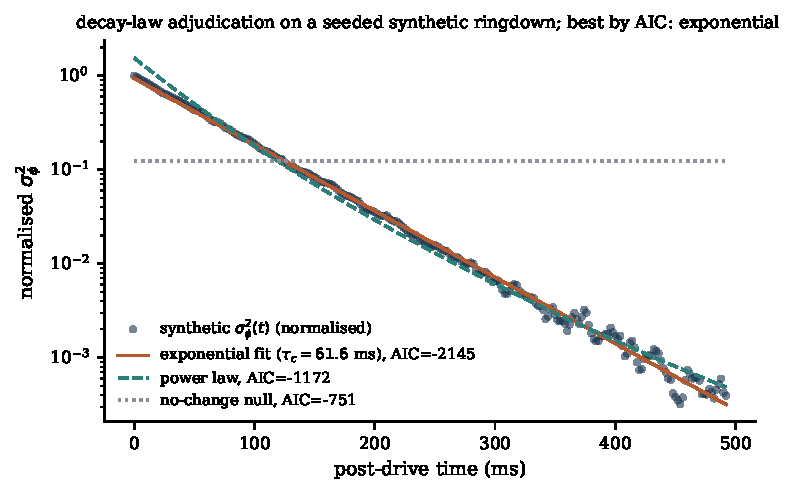
\includegraphics[width=0.75\linewidth]{fig_anisotropy_decay.pdf}
\caption{Anisotropy-decay model comparison \eqid{RGCS-M.54} on a seeded
synthetic three-channel ringdown with known exponential ground truth
(Derived synthetic record; analysis entirely by
\texttt{rgcs\_core.coherence}). The layout follows the three-model
comparison of \citet{gan2025}; the exponential form is adapted from their
Eq.~(6) as a fit form only, and $\tau_c$ is a bench parameter.}
\label{fig:aniso}
\end{figure}

% ======================================================================
\section{Drive systems and pulse timing}\label{sec:drive}
% ======================================================================

RGCS keeps the three archival drive branches separate; all operating
points are Source claims \SRC\ with page provenance \citep{jenhanlog},
parameterizing protocols without carrying truth value.

\paragraph{Electrode branch.} Sharp pulses near 20\,Hz (19.8 and 21\,Hz as
comparisons), $\sim$15\,V, silver electrodes at the selected node
coordinate $x_\ast$; observables are current, voltage, charge, vibration,
temperature. A nine-step progressive sequence (10--550\,Hz, Fibonacci-like
multipliers) is preserved together with its archival negative result
(Appendix~\ref{app:ledger}).

\paragraph{Sound-key branch.} Primary key 1496\,Hz (644/587\,Hz
alternates); documented macrocycle 3\,s on / 3\,s off $\times 4$ + 12\,s
pause $=$ 36\,s at one-third duty.

\paragraph{Opposed-coil branch.} Carrier 4096\,Hz, complementary
$180^\circ$ non-overlap drive, pulse widths 1--4\,\si{\micro s}, 20--60\,V,
copper/silver coils of 40+40 turns. The circuit inference at the archival
101\,mm point (60\,V, 1.3\,\si{\micro s}, 3\,A) gives $L \approx
\gvCoilL$\,\si{\micro H} and $E \approx \gvCoilE$\,\si{\micro J} \DER\ with
resistance neglected — flagged ``measure, don't infer'': inductance is
measured per coil before every campaign.

\paragraph{Exact-cycle envelope families.} The archival millisecond
prescriptions are made cycle-exact at the carrier
(Table~\ref{tab:drive}): the engineering refinements (e.g., the
half-spacing family's $\gvHalfCycles = 754+377+377$ cycles over
$\gvHalfMacroMs$\,ms) supplement, and never replace, the source-stated
values. The phase residue $r_\phi = c - \operatorname{round}(c)$ is defined
on cycle counts only; the half-spacing nominal count $\gvHalfNominal$ gives
$r_\phi = \gvResidueHalf$ cycles. Parametric bookkeeping follows
\citet{koster2026}: drive frequency, half-frequency response channel, and
observed band are three distinct recorded fields, and any response at
exactly half the drive frequency is logged as a parametric signature with
its threshold.

% Auto-generated by tools/make_tables.py from rgcs_core — do not edit.
\begin{table}[t]
\centering\small
\caption{Opposed-coil envelope families at the 4096 Hz carrier (RG-12).
Millisecond values are Source claims from the JH log; the exact-cycle
allocations are Derived engineering refinements that do not replace the
source-stated values. The phase residue $r_\phi$ is defined on cycle counts
only (D-13).}
\label{tab:drive}
\begin{tabular}{@{}lcccccc@{}}
\toprule
family & ON/spacing/pause (ms) & macro (ms) & duty & nominal cycles &
exact allocation & $r_\phi$ \\
\midrule
standard & 46 / 46 / 184 & 552 & 0.3333 & 2260.992 & 2261 = 754+754+753 & -0.008 \\
half spacing & 46 / 23 / 92 & 368 & 0.5000 & 1507.328 & 1508 = 754+377+377 & +0.328 \\
double rate & 23 / 23 / 92 & 276 & 0.3333 & 1130.496 & 1131 = 377+377+377 & +0.496 \\
\bottomrule
\end{tabular}
\end{table}


% ======================================================================
\section{Experimental protocols and controls}\label{sec:protocols}
% ======================================================================

\subsection{The common measurement contract}

Every branch inherits a binding contract (protocol \S0), modeled on the
measurement chain of \citet{koster2026}:

\begin{enumerate}
\item \textbf{Shared reference clock.} All generation and detection
instruments lock to one reference; the derivation is recorded per run.
Phase or coherence claims from unshared-clock runs are non-compliant.
\item \textbf{Single-shot I/Q.} No averaging across excitation cycles
before coherence analysis; each shot is stored individually.
\item \textbf{$N \ge 100$ runs} before any ensemble-phase statement
(Koster et al.\ used 1{,}000; $N$ is recorded per campaign).
\item \textbf{Acquisition $\ge 2.5\times$ past drive-off} for any
coherence claim — post-drive evolution can carry the strongest ordering
signal; runs below the ratio are amplitude-only.
\item \textbf{Controls precede attribution.} Instrument-only and
no-specimen controls at identical settings must be complete before any
coherence or enhancement claim (Figure~\ref{fig:controls}).
\item \textbf{Coherence triplet.} Every coherence value ships as
$(\Cw, w, b_w)$, always alongside an amplitude report.
\item \textbf{Sensor geometry per run.} Position and aperture of every
sensor are first-class metadata; the aperture is a spatial low-pass filter
on mode shapes.
\item \textbf{Artifact register.} Known instrument artifacts (frequencies,
conditions) are listed per campaign and referenced from every manifest.
\item \textbf{Thresholds are apparatus-specific.} No threshold from any
other apparatus — in particular the 21\,dBm value of
\citet{koster2026} — is ever a bench target or comparison point.
\item \textbf{Vocabulary.} Multi-channel disagreement metrics are
\emph{spatial phase anisotropy}; no condensation or dark-sector vocabulary
for RGCS quantities.
\end{enumerate}

Calibration gates precede every hypothesis test: instrument phase-drift
budget; coherence baseline $b_w$ with window-sensitivity scan;
known-weak-tone injection establishing amplitude and coherence detection
floors (which makes null claims quantitative); dated sensor calibration;
and correction-ledger stability. Statistics are estimation-first — effect
sizes $G_c$ and $d_c$ with seeded bootstrap confidence intervals
\citep{efron1979} — with verdict-style tests pre-registered at
$\alpha = 0.05$ under per-family Benjamini--Hochberg control
\citep{benjamini1995}, blinded analysis with hash-committed freezes, and
scrambled-label nulls against look-elsewhere effects.

\subsection{The eight branches}

Table~\ref{tab:protocol} summarizes the eight pre-registered branches;
Figure~\ref{fig:controls} shows the control matrix. Three boundaries are
absolute. \textbf{Human loading (Branch 5) is a non-clinical bench
procedure}: a volunteer holds an undriven crystal; ethics review (or
documented exemption) is required before any participant contact; no
physiological measurement, health-related claim, or therapeutic framing is
permitted in any artifact; no drive is ever energized during human contact
(hardware-interlocked). \textbf{The water branch (Branch 7) is
exploratory}: it is pre-registered as estimation-only adversarial
replication, tied to no H-xx hypothesis; any positive finding generates a
new pre-registration and can never retroactively support existing
hypotheses. \textbf{Control-subtracted metrics carry the evidence}: the
fractional gain $G_c = \max(0, (\bar Y_{\rm cfg} - \bar Y_{\rm ctl})/\bar
Y_{\rm ctl})$ and standardized effect size $d_c$ \eqid{RGCS-M.57}\ \EST\
are computed against dummy-load, no-crystal, and detuned
($\epsilon = 1.25$ convention) controls; the engineering merit
$S = |\Lambda|^2 D_f P_\phi N_x G_c$ \eqid{RGCS-M.58}\ \DER\ ranks
configurations for replication priority and is never evidence.

% Auto-generated by tools/make_tables.py from rgcs_core — do not edit.
\begin{table}[t]
\centering\small
\caption{Pre-registered experimental branches (EXPERIMENT\_PROTOCOL v1.0.0).
Every branch inherits the \S0 contract: shared reference clock, single-shot
I/Q, $N \geq 100$ runs before ensemble-phase claims, acquisition
$\geq 2.5\times$ past drive-off, controls before attribution, coherence
triplet reporting, per-run sensor geometry, artifact register,
apparatus-specific thresholds.}
\label{tab:protocol}
\begin{tabular}{@{}p{0.13\linewidth} p{0.24\linewidth} p{0.27\linewidth} p{0.27\linewidth}@{}}
\toprule
branch & hypotheses & primary observables & key controls \\
\midrule
1 modal survey & H-01, H-01a, H-03, H-04, H-07, H-09 (partial) & $f_n$, $Q_n$, $\gamma_n$, $\hat x_e$, parity phases & fixture-only; glass dummy; reference resonator \\
2 electrode pulse & H-14 (primary), H-12, H-13, H-11 & $G_c$, $d_c$, $(\mathcal{C}_w, w, b_w)$, $Z_R$, $\tau_c$ & shielded RC dummy; dummy electrodes; sham; injection \\
3 sound key & H-02 (primary), H-12, H-14, H-11 & $\epsilon$-resolved $d_c$; key vs matched off-key & speaker-only; matched-SPL off-key; muted sham \\
4 opposed coil & H-14 (primary), H-09, H-10, H-12, H-13, H-11 & mode-band I/Q; ring-up/ringdown envelopes; $\tau_c$ & no-crystal coils; resistor dummy; rotated coil \\
5 human loading & H-08, H-08b & $k_H$ per mode; repeatability variance; $\Delta M_H$ & fixture/surrogate loads; calibrated masses; ethics gate \\
6 spiral cone & H-06, H-06a, H-05 & apex-band $G_c$, $d_c$; fitted $\kappa_\chi$ vs priors & disk, plain cone, Archimedean, flat log spiral \\
7 water & none (exploratory) & pre/post chemistry deltas; blinded photo scoring & sham; thermal; evaporation; crystal-absent; ultrasonic \\
8 spatial mapping & H-03, H-10, H-11, H-13 & $\sigma_\phi^2(t)$, $\Sigma_\phi$, $\bar\Sigma_\phi(t)$; PLV & rigid dummy bar; common injection; channel scrambling \\
\bottomrule
\end{tabular}
\end{table}


\begin{figure}[t]
\centering
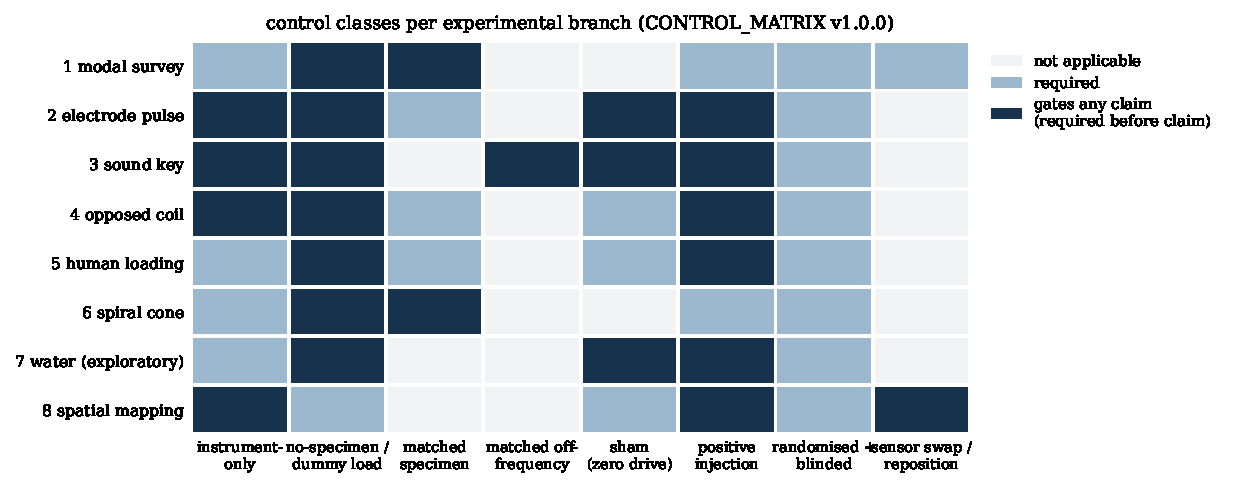
\includegraphics[width=0.98\linewidth]{fig_control_matrix.pdf}
\caption{Experimental control matrix. Dark cells are
\emph{required-before-claim} gates: an analysis on that branch fails QA if
the control is not complete at identical settings. The matched-SPL
off-frequency class is the decisive test of any ``key'' claim; positive
injection establishes the detection limits that make null results
quantitative.}
\label{fig:controls}
\end{figure}

% ======================================================================
\section{Worked examples generated from code}\label{sec:examples}
% ======================================================================

Every number in this section (and throughout the manuscript) is computed at
build time by \texttt{rgcs\_core}~2.0.0 \citep{rgcscore2026} via
\texttt{tools/make\_figures.py} and \texttt{tools/make\_tables.py}; nothing
is hand-copied. Table~\ref{tab:golden} reproduces the project's golden
reference values; Table~\ref{tab:goldencoh} re-analyses the golden
coherence datasets from their CSVs.

\paragraph{Example 1 — exact pair resonance.} $f_x = 20480$\,Hz, $p = 2$,
$f_m = 40960$\,Hz $\Rightarrow$ $\epsR = 0$ exactly. The experimental
question is then whether two measured families actually occupy those
frequencies, exhibit nonzero overlap $\Lambda$, and show splitting or
control-surviving transfer gain when swept through the condition
(H-02); Table~\ref{tab:classes} shows how quickly the class degrades with
detuning at realistic $Q$.

\paragraph{Example 2 — the ambiguous 116\,mm specimen.}
Section~\ref{sec:ladder} and Table~\ref{tab:worked}: $N_{\rm eff} =
\gvNeffOneSixteen$, class set $\gvClassSetOneSixteen$. RGCS treats this as
a calibration problem — wave-speed anisotropy, mixed modes, fixture
stiffness, and measured peaks decide the assignment, not proximity
arithmetic.

\paragraph{Example 3 — spiral prior versus placeholder.} The spiral
default geometry gives $\ell_{3D} = \gvEllThreeD$\,mm and
$R_\chi^{(s)} = \gvRchiPrior$\,mm, hence a prior slope $\kchi \approx
\gvKappaPrior$\,Hz — versus $\gvKappaChi$\,Hz for the 100\,mm placeholder.
The pre-registered fit (H-06a) asks whether either spiral prior (mean or
per-turn) falls within the $\kchi$ interval fitted from measured spacing,
against the scrambled-index null.

\paragraph{Example 4 — loading.} $k_H = \gvKH$, $\Delta M_H = \gvDMH$\,g
at $\eta = 0.5$ (Section~\ref{sec:node}) — quotable only with the $\eta$
caveat or after the two-loading protocol.

\paragraph{Example 5 — dynamic pipeline on synthetic ground truth.}
Figures~\ref{fig:cohamp}--\ref{fig:aniso} and Table~\ref{tab:goldencoh}:
the coherence metric recovers unity on a pure tone
($\min \Cw = \gvCaseBCoh$), sits at the predicted baseline on white noise
($\langle\Cw\rangle = \gvCaseACoh$ vs $b_w = \gvBaselineNw$), detects order
below the amplitude floor, distinguishes spontaneous from drive-imprinted
ensembles, and the decay-law comparison recovers a known $\tau_c$ within
$3\%$. These are software verifications \DER\ — necessary before first use
on data, evidential about nothing physical.

% Auto-generated by tools/make_tables.py from rgcs_core — do not edit.
\small
\begin{longtable}{@{}l p{0.30\linewidth} p{0.37\linewidth} p{0.15\linewidth}@{}}
\caption{Golden reference values (evidence-ledger Part E), recomputed at build
time by \texttt{rgcs\_core} 2.0.0. Ladder and compact values carry the
$\pm u_v$ systematic band of RGCS-M.10.}\label{tab:golden}\\
\toprule
ID & quantity & value (live) & label \\
\midrule
\endfirsthead
\toprule
ID & quantity & value (live) & label \\
\midrule
\endhead
G-01 & ladder constant $v_L/(2f_0)$ & 770.263671875 mm $\pm5\%$ & Derived \\
G-02 & $L_5$ & 154.052734375 mm $\pm5\%$ & Derived \\
G-03 & $L_7$ & 110.037667411 mm $\pm5\%$ & Derived \\
G-04 & $f_{ax}(110\,\mathrm{mm})$ & 28681.8182 Hz $\pm5\%$; $+9.81818$ Hz $=+0.03424\%$ vs $7f_0$ & Derived-from-Hypothesis \\
G-05 & $f_{ax}(116\,\mathrm{mm})$; class set & 27198.2759 Hz; $N_{\rm eff}=6.640204$; $\mathcal{N}=\{6, 7\}$ & Derived \\
G-06 & compact term $n{=}1$ ($v_\chi{=}\bar v_L$, $R_\chi{=}100$ mm) & 10042.6769091 Hz $\pm5\%$ & Hypothesis-conditioned \\
G-07 & $\epsilon_R^{(f)}(40960, 20480, p{=}2)$ & 0.0 (exact) & Derived \\
G-08 & hybrids for $f_A{=}f_B{=}1000$ Hz, $g{=}10$ Hz & 990 / 1010 Hz & Established \\
G-09 & $k_H(152/154.052734375)$; $\Delta M_H(154\,\mathrm{g},\eta{=}0.5)$ & 0.9866751189; 2.0937873 g & Hypothesis-conditioned \\
G-10 & $a(q{=}e)$; $r\kappa$ & 0.15915494309; 0.98757049215 & Established \\
G-11 & $\arctan\sqrt{\varphi}$ vs $51.843^\circ$ & 51.8272924$^\circ$; $\Delta = -0.015708^\circ$ & Established arithmetic \\
G-12 & exact-cycle drive families (cycles) & 2261 / 1508 / 1131 & Derived \\
G-13 & coil inference (60 V, 1.3 \si{\micro s}, 3 A) & $L \approx 26$ \si{\micro H}; $E \approx 117$ \si{\micro J} & Derived (resistance neglected) \\
G-14 & electron-count correction ($10^{-14}$ A) & 62,415.09 e/s (not 2,000) & Established arithmetic \\
G-15 & shear-scalar identity $\sigma_\phi^2(\Omega,\Omega,\Omega)$ & 0.0 (exact) & Established \\
D-13 & phase residue $r_\phi(1507.328)$ & +0.328 cycles & Derived \\
\bottomrule
\end{longtable}
\normalsize


% Auto-generated by tools/make_tables.py from rgcs_core — do not edit.
\begin{table}[t]
\centering\small
\caption{Golden coherence datasets re-analysed at build time with
\texttt{rgcs\_core.coherence} ($w = 2$ ms, $N_w = 200$, hop 0.5 ms;
$b_w = (2\sqrt{\pi}/3)/\sqrt{N_w} = 0.0836$). Per-run initial phases
are the unified estimator $\varphi_0 = \arg z(0) \bmod 2\pi$
(\texttt{initial\_phase\_estimate}). All datasets are Derived
synthetic records with known ground truth; none are measurements.}
\label{tab:goldencoh}
\begin{tabular}{@{}p{0.22\linewidth} p{0.52\linewidth} p{0.17\linewidth}@{}}
\toprule
case & recomputed metrics & lesson \\
\midrule
(a) circular white noise & $\langle\mathcal{C}_w\rangle = 0.089$ vs theory $b_w = 0.084$ & baseline, not zero \\
(b) pure tone 5 kHz & $\min\mathcal{C}_w = 1.0000$; PL $= 1.0000$; $\langle f_{\rm inst}\rangle = 5000.0$ Hz & unity coherence \\
(c) decaying tone in noise & late-window $\langle\mathcal{C}_w\rangle = 0.208 > b_w$ while amplitude $\to 1.6\%$ of peak & order outlives amplitude \\
(d) 100 random-phase runs & per-run $\langle\mathcal{C}_w\rangle = 0.990$; ensemble Rayleigh $Z_R = 1.26$, $p = 0.28$ & spontaneous-order signature \\
(f) pump-leakage trap & ensemble Rayleigh $p = 6.4 \times 10^{-35}$ (uniformity rejected): drive-imprinted, Stage-III claim blocked & driven, not spontaneous \\
\bottomrule
\end{tabular}
\end{table}


Figure~\ref{fig:hierarchy} assembles the complete forward hierarchy on one
page.

\begin{landscape}
\begin{figure}[p]
\centering
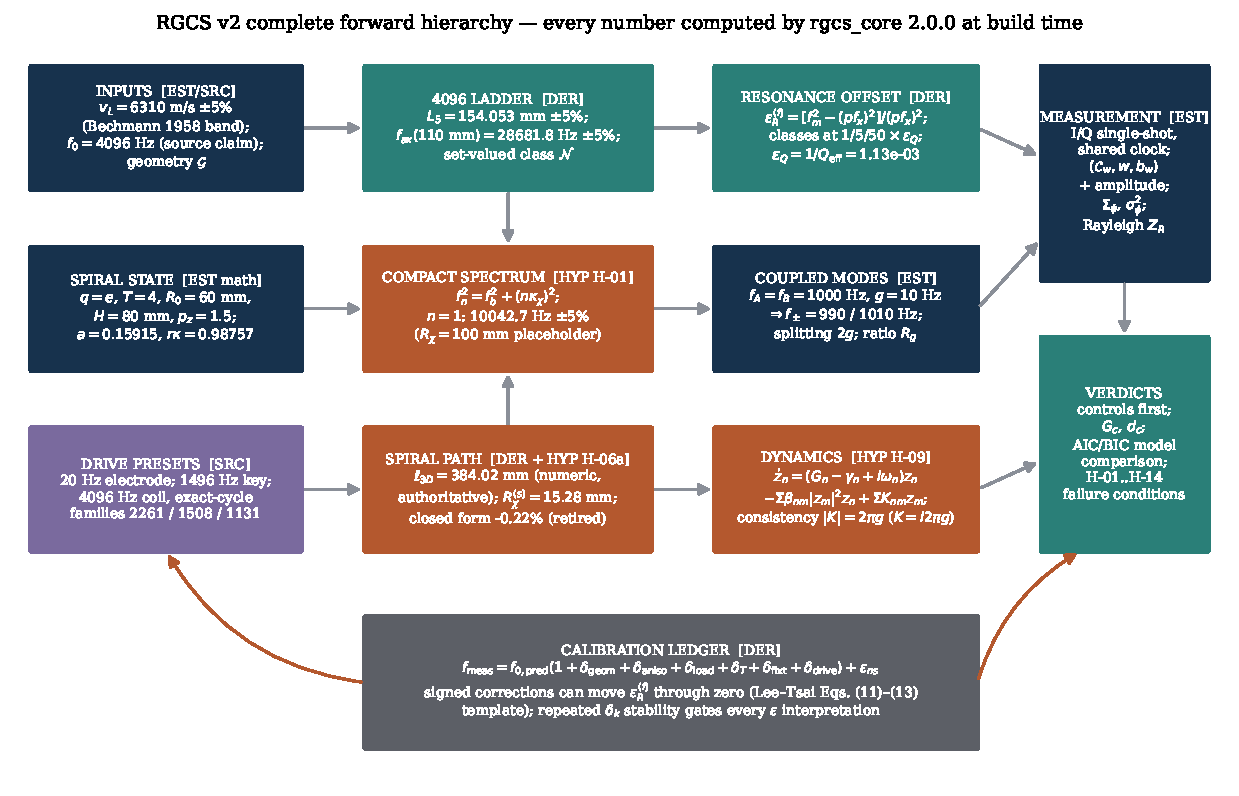
\includegraphics[width=0.98\linewidth]{fig_forward_hierarchy.pdf}
\caption{The complete RGCS v2 forward hierarchy, from declared inputs
through spectra, interaction models, and dynamics to controlled verdicts,
with the calibration ledger closing the loop. Every numerical value shown
was computed by \texttt{rgcs\_core} when this figure was generated; colors
follow the classification tags of Section~\ref{sec:scope}.}
\label{fig:hierarchy}
\end{figure}
\end{landscape}

% ======================================================================
\section{Falsification roadmap}\label{sec:roadmap}
% ======================================================================

Every Hypothesis-classified element ships with an observable, controls, a
pre-registered failure condition, and its dominant uncertainty. All
fourteen start \emph{untested}; H-14's inputs are archival negative
results. The roadmap is binding: no post-hoc bin, window, or criterion
changes.

\small
\begin{longtable}{@{}l p{0.40\linewidth} p{0.44\linewidth}@{}}
\caption{Pre-registered hypotheses and failure conditions (abridged from
the falsification roadmap; protocol branches in
Table~\ref{tab:protocol}).}\label{tab:roadmap}\\
\toprule
ID & hypothesis & pre-registered failure condition \\
\midrule
\endfirsthead
\toprule
ID & hypothesis & pre-registered failure condition \\
\midrule
\endhead
H-01 & compact spectrum $f_n^2 = \fb^2 + (n\kchi)^2$ describes a measured
family & fails to beat linear ladder, plate law, and per-mode fit on
held-out RMS/AIC, or survives index scrambling no better than chance \\
H-01a & 1-D half-wave applies to faceted crystals & majority of specimens
outside $f_{ax}(1 \pm \uv)$ \\
H-02 & enhancement localizes near $\epsR = 0$ & no localized $d_c$
increase in the within-linewidth band vs the far band at pre-registered
$\alpha$ \\
H-03 & parity families are measurable and boundary-derived & assignments
not reproducible across sensor placements, or indistinguishable from a
random partition \\
H-04 & zero-mode structure matches the declared flag & measured symmetric
family contradicts the flag (records the Lee--Tsai analogy as partial) \\
H-05 & coupling scales as $g \propto (2\pi\Rchi)^{-1/2}$ & measured ratio
differs from $\sqrt{R_2/R_1}$ beyond $2\sigma$ \\
H-06 & spiral cone outperforms matched controls & fails to beat
\emph{every} matched control (disk, plain cone, Archimedean, flat log
spiral) on the single pre-registered observable \\
H-06a & the spiral path is the compact path & neither spiral prior falls
in the fitted $\kchi$ interval, or the per-mode fit wins without penalty \\
H-07 & functional node sits at the shaft-midpoint prior $x_g$ &
$|\hat x_e - x_g| > 2\sigma_x$ reproducibly ($\hat x_e$ then supersedes
regardless) \\
H-08 & loading is first-order added modal mass & shifts not repeatable
within tolerance; or $k_H > 1$ observed; or $\Delta M_H$ inconsistent
across modes \\
H-08b & $\tilde k_H \approx k_H$ & $|\tilde k_H - k_H| > u(k_H)$ — the
proxy is retired to a design heuristic \\
H-09 & amplitude--phase dynamics \eqref{eq:sl} describe ring-up,
saturation, interaction & linear null fits saturation data as well
($\Delta\mathrm{AIC} < 2$); or $|K_{nm}| \neq 2\pi g_{nm}$ beyond $2\sigma$ \\
H-10 & anisotropy relaxes exponentially with time constant $\tau_c$ &
exponential not preferred over the no-change null by
$\Delta\mathrm{AIC} \ge 4$, or $\tau_c$ unstable across repeats \\
H-11 & $\tau_c$ is drive-branch independent at matched energy & branch
values differ beyond combined fit uncertainty — $\tau_c$ reclassified as
a calibration term \\
H-12 & coherence shows threshold-then-saturation vs drive power & no
reproducible change point across the available range (day-replication
required for any threshold claim) \\
H-13 & ordered response is spontaneous, not drive-imprinted & ensemble
phase locks to drive phase (Rayleigh $p < \alpha$) — the response is
driven \\
H-14 & coherence re-adjudication of archival amplitude-nulls & if
coherence is also null at the measured detection limit, the negative
results upgrade to ``amplitude-null AND coherence-null''; either outcome
replaces the current incomplete label \\
\bottomrule
\end{longtable}

What is \emph{not} a hypothesis: the significance of $f_0 = 4096$\,Hz
(Source claim; no experiment here can confirm numerological significance);
Established mathematics (verified by golden-value unit tests, not
experiments); and the source presets themselves (they parameterize
protocols, carrying no truth value).

% ======================================================================
\section{Limitations}\label{sec:limitations}
% ======================================================================

\begin{enumerate}
\item \textbf{Every hypothesis is untested.} This manuscript contains no
supported physical claim beyond Established mathematics and measurement
technique; it is a framework plus a test programme.
\item \textbf{The 1-D modal models are first-order.} Real quartz modes are
coupled, anisotropic, and sensitive to cut, mounting, surface state, and
electrodes \citep{xie2022,hu2025,emser2024,luo2026}; the $N$-mode
eigenproblem is a near-degenerate weak-coupling model, not elastodynamics.
Finite-element and impedance-spectroscopy validation is the intended next
stage.
\item \textbf{The wave-speed band dominates.} At $\uv = 0.05$ every
length--frequency statement is a $\pm 5\%$ interval; harmonic classes are
set-valued; no sub-percent match can mean anything until specimen
orientation is measured and $\uv$ shrinks.
\item \textbf{Identifiability limits are structural.} $(\vchi, \Rchi)$
degenerate to $\kchi$; $(\eta, \Delta M_H)$ degenerate in single-loading
data; $(G_n, \gamma_n)$ separable only with independent ringdowns;
$(\beta_{nm}, K_{nm})$ require power sweeps plus two-tone data.
\item \textbf{The dynamic model is a normal form.} Eq.~\eqref{eq:sl} is
the weakest structure producing threshold, locking, and ringdown; it is
not a kinetic equation and makes no thermalization claim.
\item \textbf{Analogies are mathematical only.} The three papers supply
equations and methods; their physics is not imported, and several of their
central concepts are deliberately not adapted
(Appendix~\ref{app:ledger}).
\item \textbf{Pilot-scale statistics.} All repeat counts are honest
precision arguments, not confirmatory power claims; no prior effect sizes
exist for any RGCS hypothesis, so first campaigns estimate the variances
that future power calculations will consume.
\item \textbf{Source corpus quality.} The archival corpus is non-peer-reviewed,
contains arithmetic errors (some corrected here as worked examples), and
its claims enter only as provenance-tracked Source claims.
\end{enumerate}

% ======================================================================
\section{Reproducibility and software}\label{sec:software}
% ======================================================================

The computational core \texttt{rgcs\_core}~2.0.0 \citep{rgcscore2026} is a
deterministic, typed Python library (numpy/scipy/pydantic) implementing
equations RGCS-M.0--M.61 with: classification metadata on every
claim-bearing public function (machine-checked); a forbidden-vocabulary
lint; JSON serialization in which NaN/$\infty$ always become \texttt{null};
seeded randomness only; and unit conversions appearing exactly once per
function. The test suite comprises 227 automated tests: 118 unit tests,
17 property-based suites (spectrum monotonicity, eigenvalue interlacing,
circular-statistic bounds, shear-scalar invariances), 19 golden-value
tests reproducing Table~\ref{tab:golden}, 50 regression tests (every
expected value of the golden coherence manifest recomputed from the CSVs,
generator determinism, the corrected time--frequency coupling map), plus
10 desktop integration tests and 13 UI smoke tests.

This manuscript is itself a reproducibility artifact: {\ttfamily
tools/make\_figures.py} and {\ttfamily tools/make\_tables.py} import
\texttt{rgcs\_core} from the repository, regenerate every figure (vector
PDF), every table, and every inline numerical macro used above, and the
document is compiled with \texttt{latexmk -xelatex}. Reviewing agents are
expected to recompute all examples. Experiment data schemas (run manifest,
specimen, environment, analysis result), the control-matrix JSON, branch
templates, and the pre-registered statistical analysis plan live alongside
the code; analyses are re-runnable from manifests alone. CAD generators
\citep{greenscad2026,greenspiralscad2026} embed the same constants with
classification-labeled headers.

% ======================================================================
\section{Conclusion}\label{sec:conclusion}
% ======================================================================

RGCS v2 turns a source-audit programme into one coherent eigenmode,
dynamics, and calibration system. The 4096 ladder supplies an axial design
family carried honestly inside its $\pm 5\%$ wave-speed band \DER. The
spiral supplies a scale-rotation path whose authoritative numeric length
feeds two competing compact-radius priors \DER/\HYP. Lee and Tsai's
architecture supplies — as mathematics, with the substitution map stated
at every use — a compact-mode spectrum, parity families with an explicit
zero-mode flag, a signed resonance offset with corrections that can move
it through zero, and a coupling-scaling test \HYP\ \citep{leetsai2026}.
Coupled-mode theory supplies hybrid eigenvalues and the avoided-crossing
signature \EST. Gan et al.\ supply the anisotropy scalar and the
decay-law adjudication methodology \citep{gan2025}; Koster et al.\ supply
the phase-referenced single-shot architecture, the coherence metric and its
triplet reporting rule, and the spontaneity test \citep{koster2026} \EST.
The JH audit supplies drive branches, node-placement requirements, source
presets, and preserved negative results \SRC. Fourteen pre-registered
hypotheses with failure conditions, eight control-gated experimental
branches, and a build system in which every number is regenerated from the
tested core give the programme its verdict mechanism. The final word
belongs to control-subtracted data: \emph{physical correspondence is
determined by measurement, not assumed by terminology.}

\bibliographystyle{unsrtnat}
\bibliography{references}

\appendix

% ======================================================================
\section{Notation and units (frozen)}\label{app:notation}
% ======================================================================

Single-owner base letters (never reused bare): $p$ (pair multiple), $a$
(spiral pitch), $Q$ (quality factor), $S$ (merit score), $q$ (spiral
growth ratio), $\rho$ (density), $L$ (crystal length), $g$ (two-mode
coupling), $n$ (compact/parity index), $N$ (axial harmonic index). Bare
$\sigma$ is forbidden ($\sigma_x$, $\sigma_\phi^2$, $\sigma_v$ are the
registered forms). Frequencies in Hz, angular frequencies in rad/s,
geometry in mm, wave speeds in \si{m/s}, masses in g, time in s; unit
conversions appear explicitly in equations.

\small
\begin{longtable}{@{}p{0.22\linewidth} p{0.44\linewidth} p{0.12\linewidth} p{0.12\linewidth}@{}}
\caption{Principal symbols (abridged from the frozen notation table).}\\
\toprule
symbol & definition & unit & label \\
\midrule
\endfirsthead
\toprule
symbol & definition & unit & label \\
\midrule
\endhead
$L$, $D_w$, $D_n$, $N_f$ & crystal length; wide/narrow diameters; facet count & mm, — & \EST \\
$\alpha_f$, $\alpha_m$ & female/male termination angles (per declared convention) & deg & \SRC\ (values) \\
$h_f$, $h_m$, $h_s$ & cap heights; shaft length $L - h_f - h_m$ & mm & \DER \\
$V$, $m$, $\rho$ & volume; mass; density (2.65 default) & cm\textsuperscript{3}, g, g/cm\textsuperscript{3} & \DER\ \EST \\
$\vL$, $\vbarL$, $\uv$ & wave speed as uncertain parameter; central value; relative uncertainty & \si{m/s}, — & \HYP\ \SRC\ \DER \\
$f_0$, $f_{ax}$, $L_N$, $N_{\rm eff}$, $\mathcal{N}$ & ladder base; axial estimate; ideal length; continuous class; class set & Hz, mm & \SRC\ \DER \\
$\chi$, $\Rchi$, $\vchi$, $\kchi$, $\fb$, $f_n$ & compact coordinate; radius; speed; slope $\vchi/2\pi\Rchi$; base; mode frequency & rad, mm, \si{m/s}, Hz & \HYP\ \DER \\
$P$, $n$ & parity family $\{P^-, P^+, \text{all}\}$; mode index & — & \EST\ (defn) \\
$f_m$, $f_x$, $p$, $\epsR$, $d_{\rm lin}$, $\epsilon_Q$ & bridge/target modes; pair multiple; offset; linear detuning; class scale $1/Q_{\rm eff}$ & Hz, — & \EST\ \DER \\
$\mathbf{H}$, $g$, $f_\pm$, $\vartheta_{\rm mix}$, $\Gamma_n$, $R_g$ & coupled-mode matrix; coupling; hybrids; mixing angle; FWHM linewidth; strong-coupling ratio & Hz, rad & \EST\ \DER \\
$q$, $a$, $T$, $R_0$, $H$, $p_z$, $\Omega_s$ & spiral growth; pitch; turns; outer radius; height; cone exponent; winding & —, mm & \EST\ \DER \\
$\ell_{pl}$, $\ell_{3D}$, $\ell_k$, $R_\chi^{(s)}$, $R_{\chi,k}$ & planar length; authoritative 3-D length; per-turn lengths; radius priors & mm & \EST\ \DER\ \HYP \\
$x_m$, $x_g$, $\hat x_e$, $x_\ast$, $\sigma_x$, $N_x$ & metric center; shaft-midpoint prior; measured node; selected node; scan uncertainty; alignment heuristic & mm, — & \EST\ \DER \\
$k_H$, $\tilde k_H$, $\eta$, $\Delta M_H$, $\delta_k$ & loading factor (measured); length proxy (distinct!); modal fraction; added modal mass; signed corrections & —, g & \EST\ \HYP\ \DER \\
$z_n$, $A_n$, $\phi_n$, $G_n$, $\gamma_n$, $\beta_{nm}$, $K_{nm}$ & modal amplitudes/phases; gain; damping $\omega_n/2Q_n$; saturation; coupling rate & X, s$^{-1}$ & \HYP\ \EST \\
$z$, $z_I$, $z_Q$, $\Cw$, $w$, $b_w$ & analytic signal; quadratures; coherence; window; baseline & X, s, — & \EST \\
$\Omega_j$, $\sigma_\phi^2$, $\Sigma_\phi$, $\tau_c$, $V_j$, $\bar R_j$ & per-axis phase rates; anisotropy scalar; variance tensor; relaxation time (fitted); circular variance; resultant & rad/s, s$^{-2}$, s & \DER\ \HYP\ \EST \\
$\Lambda$, $r_\phi$, $D_f$, $P_\phi$, $G_c$, $d_c$, $S$ & overlap; phase residue (cycles); detuning factor; phase closure; control-subtracted gain; effect size; merit (never evidence) & — & \DER\ \EST \\
$Z_R$, $n_s$, $\Theta$ & Rayleigh statistic; shot count; fit parameter vector & — & \EST \\
\bottomrule
\end{longtable}

% ======================================================================
\section{Derivations}\label{app:derivations}
% ======================================================================

\subsection{Added modal mass}
For a mode with effective stiffness $k_s$ and modal mass $M_{\rm eff}$,
$f \propto \sqrt{k_s/M}$; adding $\Delta M$ at the antinode with full
modal participation gives $f_{\rm loaded}/f_{\rm free} =
\sqrt{M_{\rm eff}/(M_{\rm eff} + \Delta M)} = k_H$, hence
$\Delta M_H = M_{\rm eff}(k_H^{-2} - 1)$ \eqid{RGCS-M.43}. The
conditioning (pure added mass, participation $\eta$) is Hypothesis H-08.

\subsection{Offset--detuning relation and class scale}
With $f_m = (1 + d_{\rm lin})\, p f_x$,
$\epsR = (1 + d_{\rm lin})^2 - 1 = 2 d_{\rm lin} + d_{\rm lin}^2$
\eqid{RGCS-M.19}. A pair with $Q_{\rm eff}$ has combined fractional
half-linewidth $1/(2 Q_{\rm eff})$ in $d_{\rm lin}$, i.e.\
$|\epsR| \approx 1/Q_{\rm eff} = \epsilon_Q$ at the half-linewidth —
the class unit of RGCS-M.20.

\subsection{Coherence normalization}
For the discrete windowed autocorrelation
$\mathrm{ACF}(\tau) = \sum_n z_{n+\tau}\bar z_n$ over $N_w$ samples, a
perfect tone gives $|\mathrm{ACF}(\tau)| = (N_w - |\tau|) A^2$ and
$\sum_\tau (N_w - |\tau|) = N_w^2$, so dividing by
$N_w \sum_n |z_n|^2$ normalizes the tone to exactly 1 — the discrete form
of the \citet{koster2026} normalization against a perfectly coherent
dummy signal. For circular white noise the same statistic concentrates
near $(2\sqrt{\pi}/3)/\sqrt{N_w}$, the theoretical baseline quoted with
every coherence value.

\subsection{Time--frequency coupling consistency}
For a degenerate pair coupled anti-Hermitianly,
$K_{12} = K_{21} = i\,2\pi g$ in Eq.~\eqref{eq:sl}, the linear
eigenvalues are $i(\omega_0 \pm 2\pi g)$: spectral peaks at
$f_0 \pm g$ (splitting $2g$~Hz) and an amplitude beat
$|z_1(t)| = |\!\cos(2\pi g t)|$ with node spacing $1/(4g)$. Fitted
$|K_{nm}|$ and $g_{nm}$ describing the same physics must therefore
satisfy $|K_{nm}| = 2\pi g_{nm}$ within uncertainty (pre-registered
warning flag otherwise). \emph{Erratum (this revision): the previous
requirement $K = \pi g$ with real-symmetric coupling was wrong in
structure and magnitude — real-symmetric coupling splits growth rates,
not frequencies, and would have flagged correct fit pairs as
inconsistent.}

% ======================================================================
\section{Algorithms}\label{app:algorithms}
% ======================================================================

\begin{description}
\item[Density inverse \eqid{RGCS-M.7}.] Newton iteration on
$\rho V(s_D) - m^\ast$ with analytic monotonicity guarantee, bisection
fallback, convergence $|\Delta m|/m^\ast < 10^{-10}$.
\item[Spiral path length \eqid{RGCS-M.35}.] Polyline sum over $\theta$
with $\ge 1200$ initial samples, doubling until
$|\ell^{(2s)} - \ell^{(s)}|/\ell^{(2s)} < 10^{-6}$ (Richardson-checked);
per-turn segmentation for $\ell_k$.
\item[Compact spectrum \eqid{RGCS-M.13--M.17}.] Parity index-set
generation with the zero-mode flag; mutually exclusive
($\kchi$)-vs-($\vchi, \Rchi$) parameterizations; first-order uncertainty
propagation to every mode.
\item[$N$-mode eigenproblem \eqid{RGCS-M.28}.] Symmetric validation
(zero diagonal, $g_{nm} = g_{mn}$), \texttt{numpy.linalg.eigh}.
\item[Stuart--Landau integration \eqid{RGCS-M.46}.] Complex-form
Euler--Maruyama with exponential integrating factor for the stiff linear
part; seed required whenever noise $> 0$; amplitude and phase returned
separately.
\item[Coherence series \eqid{RGCS-M.56}.] Sliding boxcar
($w$, hop declared), per-window FFT autocorrelation, tone-normalized;
baseline theory $(2\sqrt{\pi}/3)/\sqrt{N_w}$.
\item[Windowed phase rates / anisotropy \eqid{RGCS-M.51--M.53}.]
Unwrapped-phase least-squares slope per window (normative estimator);
scalar and tensor reductions; common-injection validation control.
\item[Model comparison \eqid{RGCS-M.60}.] Four fixed models
(exponential, power law, damped oscillatory, no-change), full AIC/BIC
table always published; ties at $\Delta\mathrm{AIC} < 2$; scrambled-label
permutation nulls ($\ge 1000$ seeded permutations) for spectra and parity.
\item[Threshold detection.] Midpoint-crossing estimator with seeded
bootstrap CI; day-replication required before any threshold claim.
\end{description}

% ======================================================================
\section{Source-claim ledger, traceability, and negative results}\label{app:ledger}
% ======================================================================

\subsection{Adapted-mathematics traceability matrix}

\small
\begin{longtable}{@{}p{0.17\linewidth} p{0.23\linewidth} p{0.24\linewidth} p{0.11\linewidth} l@{}}
\caption{Paper-to-system traceability with classification. Every adapted
equation states its substitution map at point of use; ``validation''
names the measurement that would support or kill the row.}\label{tab:trace}\\
\toprule
paper element & source role & RGCS adaptation & validation & label \\
\midrule
\endfirsthead
\toprule
paper element & source role & RGCS adaptation & validation & label \\
\midrule
\endhead
\multicolumn{5}{@{}l}{\emph{Lee \& Tsai \citep{leetsai2026}. Maps $m \to f$, $m_B \to \fb$, $1/R \to \vchi/2\pi\Rchi$; zero-mode flag stated at every use.}}\\
compact coordinate (orbifold $y$, radius $R$) & dark-sector compactification & closed wave path $\chi$, fitted $\Rchi$ (via $\kchi$) & fitted spacing, H-01 & \HYP \\
KK towers, Eqs.~(9)--(10) & tree-level mass spectra & Eq.~\eqref{eq:compact} & held-out prediction & \HYP \\
BC parity, Table~I, Eqs.~(1)--(2) & orbifold mode selection & $P^\pm$ families + \texttt{include\_zero\_mode} & two-sensor phase, H-03/H-04 & \EST\ (math) \\
resonance level, Eq.~(13) & mediator-pair offset & $\epsR$, Eq.~\eqref{eq:epsf}, same sign convention & sign-resolved sweep, H-02 & \DER \\
loop corrections, Eqs.~(11)--(12) & signed mass shifts & signed correction ledger $\delta_k$ & ledger stability & \DER \\
coupling reduction, Eq.~(6) & $g_1 = g_1^{(5)}/\sqrt{L}$ & $g \propto (2\pi\Rchi)^{-1/2}$ & refit after geometry change, H-05 & \HYP \\
$\epsilon_R = 1.25$ contour & their non-resonant reference & far-detuned \emph{control convention} only & control runs & \DER\ (conv.) \\
\multicolumn{5}{@{}l}{\emph{Gan et al.\ \citep{gan2025} — map: $H_i \to \Omega_j$}}\\
shear scalar, Eq.~(2) & Bianchi-I anisotropy measure & $\sigma_\phi^2$, Eq.~\eqref{eq:shear} (bench statistic) & golden identities; common-injection control & \EST\ (defn) \\
kinematic decomposition & expansion/vorticity/shear & mean rate $\Theta_\phi$ reported beside $\sigma_\phi^2$ & three-channel data & \DER \\
exponential decay, Eq.~(6) & post-bounce shear damping & $M_{\exp}$ fit form; $\tau_c$ bench-fitted & AIC/BIC set, H-10 & \HYP\ (form cited) \\
matter independence & five matter models, same exponent & branch-independence of $\tau_c$ as test design & matched-energy branches, H-11 & \HYP \\
three-model comparison & GR/LQC/mLQC-I layout & null/power/exponential comparison plots & COH-M14 & \EST\ (method) \\
\multicolumn{5}{@{}l}{\emph{Koster et al.\ \citep{koster2026}}}\\
I/Q single-shot chain & phase-referenced detection & measurement contract \S\ref{sec:protocols} & instrument budget & \EST \\
autocorrelation coherence & Methods metric & $\Cw$, Eq.~\eqref{eq:coherence}, triplet rule & golden cases (a)--(c) & \EST \\
1{,}000-shot phase ensembles & spontaneity evidence & Rayleigh $Z_R$ protocol, H-13 & $n_s \ge 100$ ensembles & \EST\ (method) \\
threshold behavior & pump-power onset & change-point + day-replication, H-12 & power sweeps & \HYP \\
sub-amplitude coherence & remanence below noise floor & null re-adjudication rule, H-14 & detection-limit injection & \DER\ (rule) \\
parametric $f/2$ pumping & pair injection & bookkeeping fields; parametric branch terms (off by default) & $f/2$ response logging & \DER \\
aperture spatial filtering & antenna as low-pass & sensor aperture metadata + correction concept & sensor-placement sweep & \EST \\
\bottomrule
\end{longtable}

\subsection{Not adapted (binding exclusion lists)}

\textbf{From Lee \& Tsai:} relic abundance and freeze-out; kinetic-mixing
values $\kappa$; axial-vector DM coupling; direct-detection cross-sections;
SN1987A bounds; the invisible/visible dark-photon distinction; decay
chains; small-scale-structure conclusions; the $10^{-8}$--$10^{-4}$ window
as anything but source context. \textbf{From Gan et al.:} the Planck-unit
coefficient $\sigma_1 \simeq 2.498\,m_{\rm Pl}$; bounce times;
Barbero--Immirzi parameter; holonomy corrections; singularity resolution;
any isotropization-of-the-universe claim. \textbf{From Koster et al.:} the
BEC/condensation interpretation as applied to any RGCS system; magnon
dispersion physics; the 281\,mT / 7.8\,GHz / 21\,dBm operating values as
targets; YIG material physics; spontaneous-symmetry-breaking claims for
RGCS responses. None of these may appear as an RGCS physical claim, code
default, or bench target.

\subsection{Preserved negative results \SRC\ (negative)}

\begin{itemize}
\item \textbf{JH-015:} the nine-step progressive electrode sequence
(10--550\,Hz) at 20/40/60\,V produced no detected acoustic response
(``no singing''). Status: \emph{amplitude-null, coherence-untested};
re-adjudication is Branch 2 / H-14.
\item \textbf{JH-031:} plant-stimulation test at 100\,V / 300\,ns: no
effect reported. Status: \emph{amplitude-null, coherence-untested}.
\item \textbf{JH-033:} minute charge-amplifier signals in the 101\,mm coil
configuration were attributed by the source to drive pickup. Status:
pickup floor; the no-crystal energized-coil control of Branch 4 makes this
subtraction mandatory before any coil-branch claim.
\end{itemize}

\subsection{Numerology containment \EST\ (arithmetic) / \SRC\ (significance)}

The powers-of-eight ladder ($64 \cdot 8^{n-1}$, 4096 at level 3), the
2.45\,GHz ratio decoding, and the golden-angle candidates are preserved as
audited arithmetic with corrections of source typos; the angle audit gives
$\arctan\sqrt{\varphi} = \gvAngleGolden^\circ$ against the proposed
$51.843^\circ$ ($\Delta = \gvAngleDelta^\circ$, quantified and nonzero).
No physical inference is drawn from any of it, and the scrambled-label
null of the statistical plan exists precisely to kill nearest-integer
coincidence hunting.

\end{document}
